\documentclass{article}
\usepackage{amsmath,amssymb,amsbsy}
\usepackage{graphicx}
\usepackage[letterpaper,lmargin=2.5cm,rmargin=2.5cm,tmargin=2.5cm,bmargin=2.5cm]{geometry}
\usepackage{color}
\usepackage{listings}
\usepackage[table]{xcolor}
\definecolor{lightgray}{gray}{0.95}
\lstset{language=Python,
        showstringspaces=false,
        frame=single,
        backgroundcolor=\color{lightgray}}
\newcommand{\xv}{\mathbf{x}}
\newcommand{\Xv}{\mathbf{X}}
\newcommand{\yv}{\mathbf{y}}
\newcommand{\zv}{\mathbf{z}}
\newcommand{\av}{\mathbf{a}}
\newcommand{\Wv}{\mathbf{W}}
\newcommand{\wv}{\mathbf{w}}
\newcommand{\tv}{\mathbf{t}}
\newcommand{\Tv}{\mathbf{T}}
\newcommand{\muv}{\boldsymbol{\mu}}
\newcommand{\sigmav}{\boldsymbol{\sigma}}
\newcommand{\phiv}{\boldsymbol{\phi}}
\newcommand{\Phiv}{\boldsymbol{\Phi}}
\newcommand{\Sigmav}{\boldsymbol{\Sigma}}
\newcommand{\Lambdav}{\boldsymbol{\Lambda}}
\newcommand{\half}{\frac{1}{2}}
\newcommand{\argmax}[1]{\underset{#1}{\operatorname{argmax}}}
\newcommand{\argmin}[1]{\underset{#1}{\operatorname{argmin}}}

\begin{document}

\title{Machine Learning in a Dynamic Game Environment}
\author{Joe Strout}
\maketitle

\noindent\hrulefill
\vspace{-5mm} %to remove some whitespace before "Contents"
\tableofcontents
\noindent\hrulefill

\section{Introduction}

Part of the ``suspension of disbelief'' when playing a game is to suppose that the non-player characters (NPCs) sharing the world with you are people, with real minds and motives.  When an NPC does something obviously unintelligent, this illusion is broken, and the player's immersion in the game is disrupted.  A common example is getting stuck on some invisible obstacle, and continuing to run or drive in place indefinitely.  An intelligent player would quickly realize the futility of that action, and try something else.

Common techniques for improving the appearance of NPC intelligence involve extensive analysis of each game level, either by a human designer or by a time-consuming offline process before the game is shipped~\cite{AIFORGAMES}.  However, many modern games (e.g. Minecraft) allow players to directly edit world terrain and mechanics, even adding logic to change the world state based on various triggers.  Offline techniques can't be used when level geometry and logic are changed in real time.

In such a dynamic game environment, machine learning (ML) techniques are needed to enable NPCs to cope effectively.  An NPC able to learn and adapt its behavior to changes in the environment can be more effective as a partner, or more challenging as an opponent.  This will make it easier for the player to maintain his or her belief in the NPCs as people with minds, increasing engagement in the game.

To explore the roles and benefits of ML algorithms in this context, a simple game was defined in which a single agent moves around a 10x10 grid (see Figure~\ref{figSampleMap}).  The environment consists of several types of obstacles: trees, walls, closed doors, and pits (with or without water).  Three kinds of objects may be found and collected: keys, which open doors; gems, which confer points; and rocks, which may be carried around and placed down.  Buttons may be found on the floor; these are pressed when the agent stands or places a rock on them.  Finally, a level may contain invisible walls; these are just like regular walls except that they are not drawn in the GUI, nor are they identified to the AI as anything other than an ordinary passable cell.

\begin{figure}
  \begin{center}
    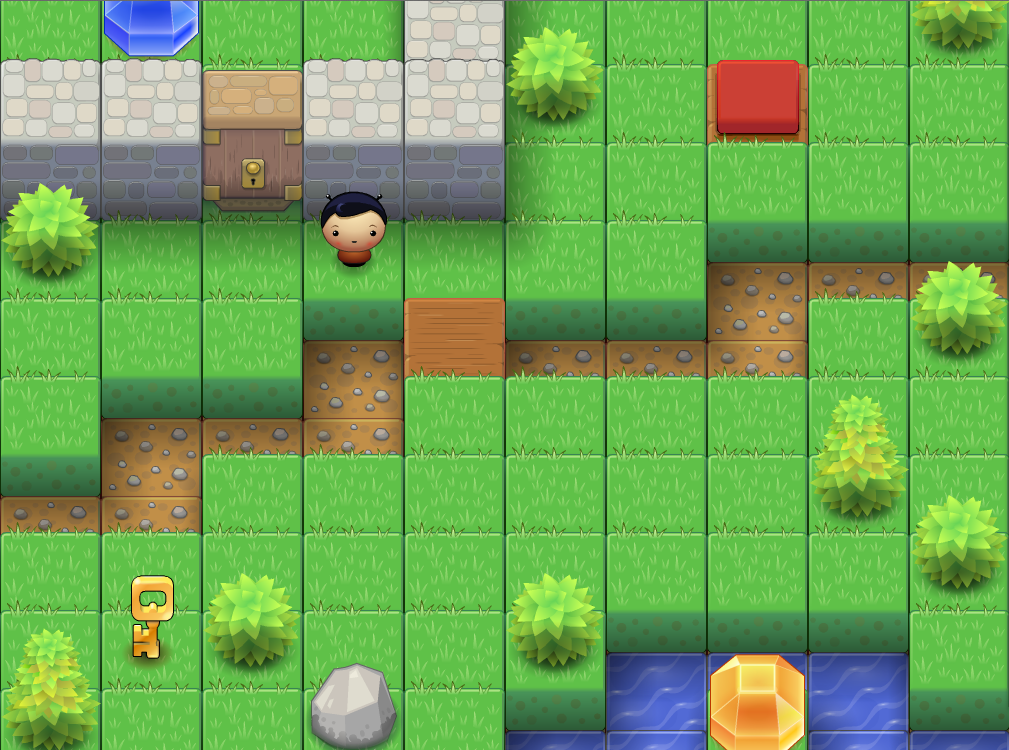
\includegraphics[width=4.5in]{figSampleMap.png}
    \caption{Game environment developed for the experiment.  Player avatar is the character just northwest of the wooden bridge.}
    \label{figSampleMap}
  \end{center}
\end{figure}

Eight different levels were designed.  Each level had unique ``level logic'' which changed the environment in response to certain events or state variables, which included the agent position, the state of any buttons on the level, and the turn counter.  This level logic was not provided in any way to the AI, nor to the human players, so any predictions about the future state of the level would have to rely solely on extrapolating from observations.  Levels were designed to simulate a variety of situations that agents might face in a real dynamic game.

Five different AIs were built and tested on these eight levels.  In addition, to provide a comparison with human gameplay, three human subjects were tested on the same levels, using a graphical representation of the game state like that shown in the figure.  These human subjects were two boys, ages 8 and 12, and one adult female with an advanced degree in computer science but relatively little experience playing computer games.  Each subject (both human and AI) was given 150 turns in each level to collect as many points as possible.  Possible actions on each turn are moving north, south, east, or west, or dropping a rock (if carrying one).  Points are awarded as follows: 25 points for each blue gem; 50 points for each green; and 100 points for each orange.

The next section of this paper will describe the architecture of the five AIs tested, including the common core decision pipeline, and the learning modules unique to each one.  Section 3 will provide implementation details, including source code for the key algorithms.  Section 4 explains each of the eight levels in more detail, and presents results for each of the eight subjects.  Finally, section 5 provides discussion and conclusions of the research.

\section{AI Architecture}

The high-level software architecture built for the AIs is shown in Figure~\ref{figArchitecture}.  The basic pipeline shown in the top row was common to all five versions of the AI.  It consists of the following:

\begin{enumerate}
\item A goal generator, which identifies key points in the map.  These include the position of gems and other collectable objects, as well as buttons.
\item A path finder, which uses a standard best-first algorithm (also known as A*) to plot a course to each goal.
\item Selection heuristics, which choose from among the reachable goals based on their expected value and path length.  When no goals are reachable, this module selects a random action.
\item The world simulation itself, which applies the result of the agent's chosen action to update the world state.
\end{enumerate}

\begin{figure}
  \begin{center}
    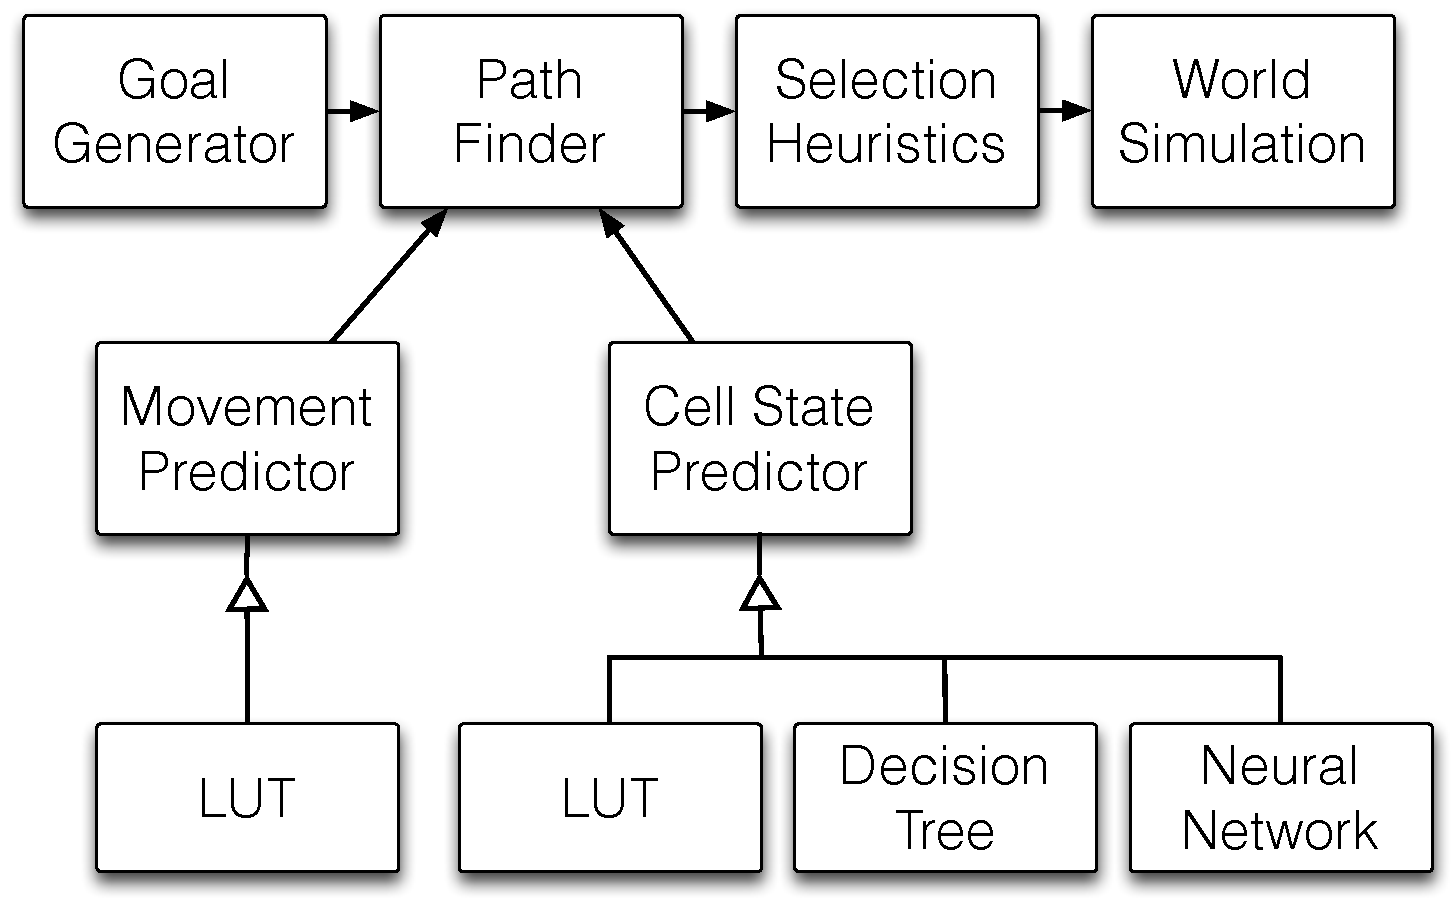
\includegraphics[width=4.5in]{figArchitecture.pdf}
    \caption{Software architecture for the agent AIs.}
    \label{figArchitecture}
  \end{center}
\end{figure}

The cycle above is then repeated for each turn.  This basic pipeline contains no learning; decisions are made solely on the observed state of the board at the moment.

To create adaptive behavior, one or two ML modules were added.  The first one is a movement predictor, tasked with guessing whether an attempted move will actually succeed.  When this module is provided, the path finder makes use of it by avoiding path steps that are predicted to fail.  The movement predictor shown in the figure is an abstract class, with one concrete implementation, based on a lookup table (LUT).  The LUT simply stores a compressed state string representing the state of the game, the attempted move, and whether that move was successful.

The second ML module added to some AIs is a cell state predictor.  This is responsible for predicting the state of the entire map, including obstacles and objects, after the agent takes some action from some previous state.  When available, the path finder uses this module's predictions, rather than assuming a static environment (apart from the direct actions of the agent).

The cell state predictor has a more difficult task, and is the central element in this study.  Three concrete implementations were prepared; all three essentially use a separate memory for each cell of the array, but they differ in the form of that memory.  The first uses a simple LUT, similar to that in the movement predictor, to predict the new state of each cell.  The second uses an incrementally updated decision tree, using the ID4 algorithm as described in~\cite{AIFORGAMES}.  The third implementation uses a neural network, updated by back-propagation using the scaled conjugate gradient (SCG) descent algorithm~\cite{CHUCKSCG}.

\section{Implementation}

All code for this study was written in Real Studio, a cross-platform, fully-compiled development environment.  This was chosen primarily because the author's eventual goal is to integrate machine learning with existing projects underway in that environment.

The full project source code is too lengthy to print here, but implementations of the key algorithms will be shown.  (Please contact the author for the full project source code.)

\subsection{Path Finding}

The most critical part of the basic AI pipeline is the the path finder.  This was implemented as a best-first search, also known as A*, using the estimated total distance to the goal to order the search nodes.  This code was based on previous work~\cite{Strout2003}, but reimplemented for this project.  Several optimizations are used to keep the number of nodes explored down, such as avoiding repeated states using a hash table; prior to those optimizations, the path finding alone could slow the entire process to a crawl.  The key method, SearchAI.FindPathTo, is shown here.

\begin{lstlisting}
Protected Function FindPathTo(game As GameState, _
            goal As MapPosition) As SearchNode
  dim startPos As MapPosition = game.PlayerChar.Position
  if startPos = goal then return nil
  
  // initialize our frontier list with a nil-action node representing
  // the start state; this will not be included on paths built from it.
  Dim nodesToExpand(0) As SearchNode
  nodesToExpand(0) = new SearchNode(game)
  nodesToExpand(0).CalcStateKey
  
  // Now, while we have work to do, pull off a node, expand it (unless we've
  // reached the maximum path length), and put its children nodes on our
  // work list.
  Dim repeatStates As New Dictionary  // key: node state key; value: true
  repeatStates.Value( nodesToExpand(0).StateKey ) = True
  Dim expandedCount As Integer
  const pathLimit = 18
  
  while nodesToExpand.Ubound >= 0
    Dim node As SearchNode = nodesToExpand(0)
    nodesToExpand.Remove 0
    for each act as Action in Action.All
      if act.Drop then
        if node.InvRocks < 1 then continue for
        if node.state.cell(node.X, 0, node.Z) _
           <> CellType.Codes.kButtonDown then continue for
      end if
      Dim nextNode As SearchNode = NextSearchNode(node, act)
      
      // Don't explore a state identical to one we've already explored.
      if repeatStates.HasKey( nextNode.StateKey ) then continue
      repeatStates.Value( nextNode.StateKey ) = True
      
      // See if we've reached the goal.
      if nextNode.X = goal.X and nextNode.Z = goal.Z then
        // found it!
        return nextNode
      end if
      
      // See if we've reached our path limit.
      nextNode.EstTotalLength = nextNode.pathLength _
         + Abs(goal.X-nextNode.X) + Abs(goal.Z-nextNode.Z)
      if nextNode.EstTotalLength > pathLimit then continue
      
      // Otherwise, insert it into our work list.
      EnqueueNode nextNode, nodesToExpand, goal
      expandedCount = expandedCount + 1
    next
  wend
  
  // No path found.
  return nil  
End Function
\end{lstlisting}

This method makes use of a helper method, EnqueueNode, the behavior of which determines whether the search is breadth-first, depth-first, best-first, etc.  The best-first implementation actually used in the project is shown here.  Note that the current implementation of this method uses a sequential search to find the correct insertion position of each node; a binary search could be considerably more efficient, and is a good opportunity for future improvement.

\begin{lstlisting}
Protected Sub EnqueueNode(node As SearchNode, queue() As SearchNode,
       goalPos As MapPosition)
  // Enqueue the given node into the search list.
  // Nodes will be expanded from the queue starting with item 0.

  // Best-first search (aka A*)
  // Insert into the queue, ordered by estimated total path
  // length to the goal    
  Dim ub As Integer = queue.Ubound
  Dim i As Integer
  for i = 0 to ub
    if queue(i).EstTotalLength > node.EstTotalLength then exit for
  next
  queue.Insert i, node
End Sub
\end{lstlisting}

\subsection{Movement Prediction}

The goal generation and selection are fairly trivial, and omitted here for brevity.  The next key component of the AI is the movement predictor, built upon a base class called MovementML.  This base class has no learning at all, but instead merely reflects the hard-coded rules of the game.  It has two methods, CanMove and Train, each shown here.

\begin{lstlisting}
Function CanMove(state As CompactState, X As Integer, Z As Integer,
     dir As Integer, invKeys As Integer, invRocks As Integer,
     clock As Integer) As Boolean
  // Return whether an attempt to move as given will succeed.
  // Note that this isn't even called if the move would go out of bounds.
  
  // Let's start by looking up the target terrain and ground types.
  if state.Cell(X, 1, Z) = CellType.Codes.kDoorTallClosed then
    // A closed door is a special case: passable only if you have a key.
    return invKeys > 0
  end if
  Dim ct As CellType = CellType.GetFromCode( state.Cell(X, 1, Z) )
  Dim invdir As Integer = Direction.Opposite(dir)
  if ct <> nil and ct.BlocksMovement(invdir) then return false
  
  // Also make sure the new ground is OK to stand on.
  ct = CellType.GetFromCode( state.Cell(X, 0, Z) )
  if ct is nil or not ct.OKToStandOn then return false
  
  return true
  
End Function
\end{lstlisting}

\begin{lstlisting}
Sub Train(prevState As ExtendedState, action As Action,
      newState As ExtendedState)
  // Here's our opportunity to learn something about how the
  // world works, based on the last state, the action we took
  // in that state, and the new state after that action.
End Sub
\end{lstlisting}

The Train method, one may note, does nothing in the base class; the base class has no data.  From this was derived one subclass, MoveMLLUT, which uses a lookup table to predict the success of a movement.  This class has one property, MovementLUT as Dictionary (where Dictionary is the standard hash table implementation provided by Real Studio).  Its CanMove method uses this to override the standard, rule-based prediction provided by the superclass:

\begin{lstlisting}
Function CanMove(state As CompactState, X As Integer, Z As Integer,
      dir As Integer, invKeys As Integer, invRocks As Integer,
      clock As Integer) As Boolean
  // First, see whether we have a stored fact about this sort of movement.
  Dim extState As new ExtendedState(state, X, Z, invKeys, invRocks, clock)
  Dim fullLutKey As String = extState.LUTkey + ":" + Str(dir)
  if MovementLUT.HasKey(fullLutKey) then
    // Yep, we've tried this before... return the previous result.
    return MovementLUT.Value(fullLutKey)
  end if
  
  // No, we haven't stored any facts about this movement;
  // so just do the standard logic.
  return Super.CanMove(state, X, Z, dir, invKeys, invRocks, clock)
End Function
\end{lstlisting}

MoveMLLUT's Train method checks for cases where the actual move differs from the predicted move, and in such cases, stores a new fact in its lookup table.

\begin{lstlisting}
Sub Train(prevState As ExtendedState, action As Action,
      newState As ExtendedState)
  // Learn from unexpected results: namely, an attempt to move that failed,
  // when we expected it should succeed.
  if action.MoveDir = Direction.None then return  // no move attempt was made
  if newState.X = prevState.X and newState.Z = prevState.Z _
     and CanMove(prevState.state, prevState.X, prevState.Z, action.MoveDir, _
     prevState.InvKeys, prevState.InvRocks, prevState.clock) then
    // OK, we thought we should be able to move, but didn't.
    // Store this fact for future reference.
    Dim fullLutKey As String = prevState.LUTkey + ":" + Str(action.MoveDir)
    MovementLUT.Value(fullLutKey) = False
  end if
  
End Sub
\end{lstlisting}

Not yet shown is the source of the LUTKey method invoked by this class.  LUTKey is a method on the ExtendedState class that builds a string representation of the state of the game, including obstacles, objects, and the position of the player.  Because this was found to be a performance bottleneck, caching is used to avoid rebuilding these keys more often than necessary.  Despite that, the code is fairly simple:

\begin{lstlisting}
Function LUTkey() As String
  // Calculate a string representation of the complete extended state,
  // suitable for use in look-up tables.
  if mCachedLUTKey = "" then
    // We'll just take advantage of the debug string converter on
    // CompactState to do most of the work for us.
    mCachedLUTKey = state.DebugDump + EndOfLine _
       + Str(X) + "," + Str(Z) + " " _
       + Str(InvKeys) + " " + Str(InvRocks)
  end if
  return mCachedLUTKey  
End Function
\end{lstlisting}

Most of the work, however, is done by the DebugDump computed property on the CompactState class.  This property, as the name implies, was originally intended to provide a human-readable representation of the game state (minus player position and inventory) for debugging purposes.  But when a lookup table key was needed, it was found to be ideal for that purpose.  The code for CompactState.DebugDump is shown here.  Note that it too uses caching for performance.

\begin{lstlisting}
DebugDump.Get
  if mDebugDumpStr = "" then
    Dim lines() As String
    for z as Integer = 9 DownTo 0
      Dim codes(9*2+1) As String
      for x as Integer = 0 to 9
        select case Cell(x, 1, z)
        case CellType.Codes.kEmptyType
          if Cell(x, 0, z) = CellType.Codes.kEmptyType then
            codes(x*2) = " "
          else
            codes(x*2) = "."
          end if
        case CellType.Codes.kDoorTallOpen
          codes(x*2) = "-"
        case CellType.Codes.kDoorTallClosed
          codes(x*2) = "+"
        else
          codes(x*2) = "#"
        end select
        select case Objects(x, z)
        case ObjectType.ObjTypeCodes.kUnknownType
          codes(x*2+1) = " "
        case ObjectType.ObjTypeCodes.kKey
          codes(x*2+1) = "k"
        case ObjectType.ObjTypeCodes.kRock
          codes(x*2+1) = "o"
        else
          codes(x*2+1) = "?"
        end select
      next
      lines.Append Join(codes, "")
    next
    
    mDebugDumpStr = Join(lines, EndOfLine)
  end if
  return mDebugDumpStr
End Get
\end{lstlisting}

\subsection{Cell State Prediction: Lookup Table}

The next major part of the AI is the cell state predictor.  One predictor object is instantiated for each cell of the map, though these are intended to be very lightweight for cells that never change.  As with the movement predictor, a base class was first defined that does no learning at all.  This base class, CellML, has two key methods: NextType and Train, shown here.

\begin{lstlisting}
Function NextType(extState As ExtendedState, act As Action) As CellType.Codes
  // By default, we'll always assume no change.
  return extState.state.cell(mPosition.X, mPosition.Y, mPosition.Z)
End Function
\end{lstlisting}

\begin{lstlisting}
Sub Train(prevState As ExtendedState, action As Action,
      newState As ExtendedState)
  // Here's our opportunity to learn something about how the
  // world works, based on the last state, the action we took
  // in that state, and the new state after that action.
End Sub
\end{lstlisting}

The base class is trivial: it assumes that the next state of a cell will always equal its previous state, and its Train method does nothing.

From this base class, three different machine learning classes were derived.  The first used a simple lookup table, very similar to the MoveMLLUT class presented in the previous section.  This class, CellMLLUT, adds one property, CellTypeLUT as Dictionary.  Its NextType method uses this to infer a new state for the cell, based upon the extended state lookup key, and the movement direction of the intended action.

\begin{lstlisting}
Function NextType(extState As ExtendedState, act As Action) As CellType.Codes
  if CellTypeLUT is nil then
    // No stored facts at all for this location.  Go with the default
    // assumption of no state change.
    return Super.NextType(extState, act)
  end if
  
  Dim fullLutKey As String = extState.LUTkey + ":" + Str(act.MoveDir)
  if not CellTypeLUT.HasKey(fullLutKey) then
    // We have no fact stored for this situation, so just go with the default
    // assumption (of no change).
    return Super.NextType(extState, act)
  else
    // We've seen this cell change types in this situation before.  Report
    // what type it changed into.
    return CellTypeLUT.Value(fullLutKey)
  end if
End Function
\end{lstlisting}

The Train method is slightly more complex, because to conserve memory, it removes LUT entries that are no longer needed because they would not change the default prediction.

\begin{lstlisting}
Sub Train(prevState As ExtendedState, action As Action,
      newState As ExtendedState)
  // Any time the state changes, we'll store an entry in our LUT.
  // Any time it states the same, we'll clear that entry in our LUT.
  // (So, no entry indicates no change -- this conserves memory.)
  Dim prevType As CellType.Codes = prevState.state.cell(mPosition.X, mPosition.Y, mPosition.Z)
  Dim newType As CellType.Codes = newState.state.cell( _
       mPosition.X, mPosition.Y, mPosition.Z)
  
  Dim fullLutKey As String = prevState.LUTkey + ":" + Str(action.MoveDir)
  if prevType = newType then
    if CellTypeLUT <> nil and CellTypeLUT.HasKey(fullLutKey) then _
          CellTypeLUT.Remove fullLutKey
  else
    if CellTypeLUT is nil then CellTypeLUT = New Dictionary
    Dim prevGuess As CellType.Codes = CellTypeLUT.Lookup(fullLutKey, prevType)
    if prevGuess <> newType then
      CellTypeLUT.Value(fullLutKey) = newType
    end if
  end if
End Sub
\end{lstlisting}

\subsection{Cell State Prediction: Decision Tree}

The second of the three cell state learning algorithms uses an incremental decision tree learning algorithm, based on \cite{AIFORGAMES}.  Several data structures are involved in this implementation.  First is ID3Example, which represents a training sample.  ID3Example has two properties: actionType as Integer, which represents the output or target value of each sample; and inputs() as Double, an array of floating-point values which represent the input.  (The ID3 prefix on this classes derives from the original ID3 algorithm, of which ID4 is merely an extension.)

The next decision tree support class is ID3ExampleSet, which wraps an array of examples.  More importantly, however, it also provides an Entropy method, which calculates the entropy of its examples by calling through to a global method, ID3.Entropy, shown here.

\begin{lstlisting}
Protected Function Entropy(examples() As ID3Example) As Double
  // Computes the entropy of a set of examples.
  // This should be 0 when all examples have the same result,
  // and 1 when they are evenly distributed different results.
  // Reference: AI for Games p. 619
  
  // Get the number of examples
  Dim exampleCount As Integer = examples.Ubound + 1
  
  // Check if we only have one: in that case entropy is 0
  if exampleCount <= 1 then return 0
  
  // Otherwise, we need to keep a tally of how many of
  // each different kinds of action (result) we have
  Dim actionTallies As New Dictionary
  for each ex as ID3Example in examples
    actionTallies.Value(ex.actionType) = _
           actionTallies.Lookup(ex.actionType, 0) + 1
  next
  
  // Now we have the counts for each action in the set;
  // if we have only one action, then we have zero entropy
  if actionTallies.Count <= 1 then return 0
  
  // Otherwise, add up the contribution to entropy of each action
  static logOf2 As Double = Log(2)
  Dim result As Double
  for each actionTally As Integer in actionTallies.Values
    Dim proportion As Double = actionTally / exampleCount
    result = result - proportion * (log(proportion) / logOf2)
  next
  return result 
End Function
\end{lstlisting}

The tree structure itself consists of instances of class ID3Node, or its single subclass, ID3DecisionNode.  ID3Node is used for terminal nodes, and defines methods to look up (predict) a result given an example.  The base class implementation is trivial:

\begin{lstlisting}
Function Lookup(inputs() As Double) As Integer
  return examples.Items(0).actionType
End Function
\end{lstlisting}

Not trivial, however, is the ID3Node.Update method, which is the entry point for the ID4 algorithm.  This method adds a new fact to its growing list of examples, and when appropriate, rebuilds its part of the tree to better match the data.

\begin{lstlisting}
Function Update(newExample As ID3Example) As ID3Node
  // This method is the entry point for the ID4 (incremental decision
  // tree learning) algorithm.
  // Either update this node with the new example and return self, or
  // create a new node that includes this example and return that.
  // See AI for Games, p. 628.
  
  // This is the code for terminal nodes; decision nodes should override it.
  
  if examples.Count = 0 or examples.Items(0).actionType _
           = newExample.actionType then
    // This matches the output we already represent; just add it to our list.
    examples.Items.Append newExample
    return self
  else
    // This does not match our examples.  We need a decision node.
    examples.Items.Append newExample
    Dim grr() As Integer
    for i As Integer = 0 to examples.Items(0).inputs.UBound
      grr.Append i
    next
    Dim newbie As ID3Node = ID3.MakeTree( examples, grr )
    return newbie
  end if
End Function
\end{lstlisting}

Now let's consider ID3Node's subclass, ID3DecisionNode.  This class adds three properties: an array of two daughter nodes, a test attribute index, and a threshold.  Based on the value of the test attribute compared to its threshold, the Lookup method delegates to its left or right daughter branch.

\begin{lstlisting}
Function Lookup(inputs() As Double) As Integer
  Dim branch As Integer
  if inputs(testAttribute) > threshold then branch = 0 else branch = 1
  return daughterNodes(branch).Lookup(inputs)
End Function
\end{lstlisting}

ID3DecisionNode.Update implements the rest of the ID4 incremental update algorithm.

\begin{lstlisting}
Function Update(newExample As ID3Example) As ID3Node
  // See if the new example would cause us to make a different decision
  // than our current examples.  If not, just pass the new example on
  // down to the daughter node that already handles that type of thing.
  // But if so, then create a whole new sub-tree from here.
  
  // "Different decision" here can mean either a different attribute, or
  // a different threshold for the existing attribute.
  examples.Items.Append newExample
  
  Dim bestInformationGain As Double = 0
  Dim bestSplitAttribute As Integer
  Dim bestThreshold As Double
  Dim bestSets() As ID3ExampleSet
  
  Dim grr() As Integer
  for i As Integer = 0 to examples.Items(0).inputs.UBound
    grr.Append i
  next
  
  if not ID3.FindSplit(examples, grr, bestSplitAttribute, bestThreshold, _
        bestSets) then
    break // This should never happen.
  elseif bestSplitAttribute = testAttribute _
        and Abs(bestThreshold - threshold) < 0.0001 then
    // New example fits nicely with our current ones.  Pass it down.
    Dim branch As Integer
    if newExample.Inputs(testAttribute) > threshold then _
           branch = 0 else branch = 1
    daughterNodes(branch) = daughterNodes(branch).Update(newExample)
    return self
  else
    // New example has forced us to rethink our life a bit.
    // Create a whole new subtree.
    return ID3.MakeTree(examples, grr)
  end if
  
End Function
\end{lstlisting}

Both the Update methods can call the ID3.MakeTree method, which uses the standard ID3 algorithm to build a decision tree for a set of examples.

\begin{lstlisting}
Protected Function MakeTree(examples As ID3ExampleSet, 
        allowedAttributes() As Integer) As ID3Node
  // Create a decision tree for the given examples, 
  // considering only the given set of attributes.
  // Reference: AI for Games p. 617-618.
  
  // Find the best split for these examples
  Dim bestInformationGain As Double = 0
  Dim bestSplitAttribute As Integer
  Dim bestThreshold As Double
  Dim bestSets() As ID3ExampleSet
  if not FindSplit(examples, allowedAttributes, bestSplitAttribute, bestThreshold, bestSets) then
    Dim leaf As New ID3Node
    leaf.examples = examples
    return leaf
  end if
  
  // Set the decision node's test
  Dim decisionNode As New ID3DecisionNode
  decisionNode.examples = examples
  decisionNode.testAttribute = bestSplitAttribute
  decisionNode.threshold = bestThreshold
  
  Dim newAttributes() As Integer = allowedAttributes
  
  // Recurse for each subset
  for i as Integer = 0 to 1  // our decision nodes are always binary!
    decisionNode.daughterNodes(i) = MakeTree(bestSets(i), newAttributes)
  next
  
  return decisionNode
End Function
\end{lstlisting}

This method relies on ID3.FindSplit, which calculates the best attribute and threshold to use to divide a set of examples:

\begin{lstlisting}
Protected Function FindSplit(examples As ID3ExampleSet,
       allowedAttributes() As Integer, ByRef outAttribute As Integer,
       ByRef outThreshold As Double, ByRef outSets() As ID3ExampleSet)
       As Boolean
  // Find the best attribute (and threshold for that attribute) on
  //  which to split the given sets.  Also return the resulting split sets.
  //  Return true if successful; false if no split is called for.
  // Reference: AI for Games p. 617-618.
  
  // Calculate our initial entropy
  Dim initialEntropy as Double = examples.Entropy
  
  // No attributes or no entropy, then we can't divide further
  if initialEntropy <= 0 or allowedAttributes.UBound < 0 then return false
  
  // Find the number of examples
  Dim exampleCount As Integer = examples.Count
  
  // Hold the best split found so far
  Dim bestInformationGain As Double = 0
  Dim bestSplitAttribute As Integer
  Dim bestThreshold As Double
  Dim bestSets() As ID3ExampleSet
  
  // Go through each attribute
  for each attribute As Integer in allowedAttributes
    // Perform the split
    Dim sets() As ID3ExampleSet
    Dim threshold As Double
    SplitByContinuousAttribute examples, attribute, sets, threshold
    if sets(0) is nil then continue for
    
    // Find overall entropy and information gain
    Dim overallEntropy As Double = EntropyOfSets(sets, exampleCount)
    Dim informationGain As Double = initialEntropy - overallEntropy
    
    // Check if we've found the best so far
    if informationGain > bestInformationGain then
      bestInformationGain = informationGain
      bestSplitAttribute = attribute
      bestSets = sets
      bestThreshold = threshold
    end if
  next attribute
  
  // All done.
  outAttribute = bestSplitAttribute
  outThreshold = bestThreshold
  outSets = bestSets
  return bestSets.Ubound >= 0
  
End Function
\end{lstlisting}

Finally, for the generic decision tree code, we must example ID3.EntropyOfSets, which calculates the weighted average entropy of an array of example sets.

\begin{lstlisting}
Protected Function EntropyOfSets(sets() As ID3ExampleSet, 
        exampleCount As Integer) As Double
  // Find the entropy of the given sets of examples, which are 
  // divided up from 'exampleCount' total examples.
  // This is just the total of the entropy of each set, weighted
  // by its proportion of the total.  Put another way, it's the 
  // weighted average entropy of the sets.
  // Reference: AI for Games p. 620-621
  
  Dim entropy as Double
  for each set As ID3ExampleSet in sets
    // Calculate the proportion of the whole in this set
    Dim proportion As Double = set.Count / exampleCount
    
    // Calculate the entropy contribution.
    entropy = entropy + proportion * set.Entropy
  next  
  return entropy  
End Function
\end{lstlisting}

All this is the standard ID4 code.  Now, to tie this into the project, a subclass of CellML was defined, called CellMLDecisionTree.  It adds one property, Tree as ID3Node.  The NextType method uses this decision tree, when available, to predict the next type of its map cell:

\begin{lstlisting}
Function NextType(extState As ExtendedState, act As Action) As CellType.Codes
  if Tree is nil then
    // No memory for this location. Go with the default
    // assumption of no state change.
    return Super.NextType(extState, act)
  end if
  
  // Otherwise, use the tree to guess the new state of this cell.
  Dim sample() As Double = MakeSample(extState, act)
  return CellType.Codes(Tree.Lookup(sample))
End Function
\end{lstlisting}

The Train method creates a decision tree the first time the cell state changes, and updates it with new examples thereafter.

\begin{lstlisting}
Sub Train(prevState As ExtendedState, action As Action, 
        newState As ExtendedState)
  Dim prevType As CellType.Codes = prevState.state.cell( _
       mPosition.X, mPosition.Y, mPosition.Z)
  Dim newType As CellType.Codes = newState.state.cell(_
       mPosition.X, mPosition.Y, mPosition.Z)
  if newType = prevType and Tree is nil then
    // Common case: the type didn't change, and we didn't expect it to,
    // because we have no changes at all stored for this cell.
    return
  end if
  
  Dim sample() As Double = MakeSample(prevState, action)
  Dim newTypeInt As Integer = Integer(newType)
  if Tree is nil then
    // No decision tree previously created for this node.  Create one now.
    Dim examples As New ID3ExampleSet
    examples.Items.Append new ID3Example(sample, newTypeInt)
    Dim allowedAttributes() As Integer = Range(sample.Ubound)
    Tree = ID3.MakeTree(examples, allowedAttributes)
  else
    // Update our decision tree with the new example.
    Tree = Tree.Update(new ID3Example(sample, newTypeInt))
  end if
End Sub
\end{lstlisting}

Samples are obtained from a class inserted in the hierarchy between CellML and CellMLDecisionTree.  This class, CellMLSampler, is responsible for building an array (of type Double) that describes a state-action pair; its functionality is extracted into a superclass so that it can be reused by the neural network predictor as well.  The main method is MakeSample:

\begin{lstlisting}
Protected Function MakeSample(state As ExtendedState, action As Action) 
          As Double()
  // Build an array describing the state-action pair.  This will be used
  // as input to the decision tree.  Note that this array must be the same
  // length every time; each array element represents an input feature.
  
  Dim out() as Double = Array( _
  state.X*1.0, state.Z, _   // player character position
  state.InvKeys, state.InvRocks)   // player inventory
  
  Dim dx, dz As Integer
  if action.Drop then
    out.Append 0  // DX
    out.Append 0  // DY
    out.Append 1  // drop
  else
    dx = Direction.DX(action.MoveDir)
    dz = Direction.DZ(action.MoveDir)
    out.Append dx
    out.Append dz
    out.Append 0  // no drop
  end if
  
  // Encode the state of all buttons on the board.
  // We're going to imagine the future state of the buttons,
  // since these follow clearly-defined rules and it's their final state that
  // is likely to matter, rather than their current state.
  if not mSearchedForKeyPoints then FindKeyPoints(state.state)
  for each pos as MapPosition in mKeyPoints
    if state.X = pos.X and state.Z = pos.Z and _
      action.MoveDir <> Direction.None and _
      state.state.Objects(pos.X, pos.Z) <> ObjectType.ObjTypeCodes.kRock then
      // Player was standing on the button,
      // but is moving off (without leaving a rock)
      out.Append Integer(CellType.Codes.kButtonUp)
    elseif state.X + dx = pos.X and state.Z + dZ = pos.Z then
      // Player is about to step on the button
      out.Append Integer(CellType.Codes.kButtonDown)
    else
      out.Append Integer(state.state.Cell(pos.X, pos.Y, pos.Z))
    end if
  next
  
  // Encode the time, mod 2-10, to handle periodic changes.
  for n as Integer = 2 to 10
    out.Append state.clock mod n
  next
  
  return out
End Function
\end{lstlisting}

For the decision tree and neural network, using the entire state of the map proved cumbersome.  So instead, the feature vector encodes just the of ``key points'' in the map, currently defined as the locations of buttons and doors.  In the case of buttons, what's stored is the future state after applying the action, and assuming standard button rules; for doors (or other key points we could define), we simple store the cell type.  These key points are found by the following function:

\begin{lstlisting}
Protected Sub FindKeyPoints(state As CompactState)
  // Search the map in the given CompactState for any buttons or doors,
  // and store their locations in mKeyPoints.  These are "key points"
  // that are likely to have relevance to other things happening on the map.
  
  Redim mKeyPoints(-1)
  for x as Integer = 0 to 9
    for y as Integer = 0 to 1
      for z as Integer = 0 to 9
        select case state.Cell(x, y, z)
        case CellType.Codes.kButtonUp, _
          CellType.Codes.kButtonDown, _
          CellType.Codes.kDoorTallOpen, _
          CellType.Codes.kDoorTallClosed
          mKeyPoints.Append new MapPosition(x, y, z)
        end select
      next
    next
  next
  mSearchedForKeyPoints = true  
End Sub
\end{lstlisting}

Note that the CellMLSampler class caches the key points using the mKeyPoints and mSearchedForKeyPoints properties.  This not only improves performance, but also ensures that the number or meaning of the sample attributes does not change within a level run.

\subsection{Cell State Prediction: Neural Network}

The third and final learning algorithm used to predict cell states is based on neural network code from the CS545 course~\cite{CHUCKSCG}.  This code is based heavily around the matrix operations in the NumPy library for Python.

While Real Studio features an extensive library for GUI and multimedia work, it does not come with a matrix library.  A matrix plug-in was found~\cite{MATRIXPLUGIN}, but the semantics provided by that library turned out to be quite different from those provided by NumPy.  For example, the matrix plug-in adds a scalar to a matrix by adding it to the elements along the diagonal, whereas NumPy adds it to all elements.  To make porting NumPy-based code to Real Studio easier, an NPMatrix class was developed that implements the same semantics as 2D NumPy arrays.  The Matrix plugin is still used internally, but in the end, the only functionality actually used is matrix-matrix multiplication; all other operations were coded with loops.

While the full source code is too lengthy to print here, the following implementation of NPMatrix.Operator\_Add (which is invoked by the + operator) is representative.

\begin{lstlisting}
Function Operator_Add(rhs As NPMatrix) As NPMatrix
  // Check for compatible sizes
  Assert (M.NumRows = rhs.m.NumRows or M.NumRows=1 _
  	or rhs.M.NumRows=1) and (M.NumColumns = rhs.M.NumColumns _
  	or M.NumColumns=1 or rhs.M.NumColumns=1), _
    "Size mismatch in Operator_Add"
  
  // Compute the row and column factors, allowing a 1xM or Nx1 matrix
  // to be repeated to fit an NxM one.
  Dim leftRowFactor, leftColFactor, rightRowFactor, rightColFactor As Integer
  if M.NumRows > 1 then leftRowFactor = 1
  if M.NumColumns > 1 then leftColFactor = 1
  if rhs.M.NumRows > 1 then rightRowFactor = 1
  if rhs.M.NumColumns > 1 then rightColFactor = 1
  
  // Prepare storage for the resulting matrix.
  Dim outrows As Integer = Max(M.NumRows, rhs.M.NumRows)
  Dim outcols As Integer = Max(M.NumColumns, rhs.M.NumColumns)
  Dim out As Matrix = New Matrix(outrows, outcols)
  
  // Perform the addition, and return the result.
  Dim maxrow As Integer = outrows - 1
  Dim maxcol As Integer = outcols - 1
  for row as Integer = 0 to maxrow
    for col as Integer = 0 to maxcol
      NewElement out, row, col, _
      M.Element(row*leftRowFactor, col*leftColFactor) _
      + rhs.M.Element(row*rightRowFactor, col*rightColFactor)
    next
  next
  return New NPMatrix(out) 
End Function
\end{lstlisting}

With this NPMatrix class in hand, the code was a relatively straightforward port of Python code provided in the course.  It was divided into three classes.  First is the Optimizer class, which provides steepest-descent and scaled conjugate gradient (SCG) optimization algorithms.  Both were implemented and tested, but in the end only the SCG code was used in the project.  That function is shown below.

\begin{lstlisting}
Function SCG(x as NPMatrix, iterations As Integer) As NPMatrix
  // Scaled Conjugate Gradient algorithm.
  
  Dim nvars As Integer = x.Rows
  Dim sigma0 As Double = 1.0e-6
  Dim fold As Double = ObjectiveF(x)
  Dim fnow As Double = fold
  Dim gradnew as NPMatrix = GradientF(x)
  if gradnew.AnyNaN then break
  if NPMatrix.Dot(gradnew.T, gradnew).AsScalar = 0 then
    return x  // no gradient; already (locally) optimal
  end if
  Dim gradold As NPMatrix = gradnew
  Dim d As NPMatrix = -gradnew   // initial search direction
  Dim success As Boolean = True   // force calculation of directional derivs.
  Dim nsuccess As Integer = 0       // nsuccess counts number of successes
  Dim beta As Double = 1.0           // initial scale parameter
  Dim betamin As Double = 1.0e-15    // lower bound on scale
  Dim betamax As Double = 1.0e20     // upper bound on scale
  Dim j As Integer = 1  // j counts number of iterations
  Dim mu, theta, kappa As Double
  
  // Main optimization loop.
  for j = 1 to iterations
    
    // Calculate first and second directional derivatives.
    if success then
      mu = NPMatrix.Dot(d.T, gradnew).AsScalar
      if NPMatrix.IsNAN(mu) then break
      if mu >= 0 then
        d = -gradnew
        mu = NPMatrix.Dot(d.T, gradnew).AsScalar
      end if
      kappa = NPMatrix.Dot(d.T, d).AsScalar
      Dim sigma As Double = sigma0 / sqrt(kappa)
      Dim xplus As NPMatrix = x + sigma * d
      Dim gplus As NPMatrix = GradientF(xplus)
      theta = NPMatrix.Dot(d.T, gplus - gradnew).AsScalar / sigma
    end if
    
    // Increase effective curvature and evaluate step size alpha.
    Dim delta As Double = theta + beta * kappa
    if delta <= 0 then
      delta = beta * kappa
      beta = beta - theta/kappa
    end if
    Dim alpha As Double = -mu / delta
    
    // Calculate the comparison ratio.
    Dim xnew As NPMatrix = x + alpha * d
    if xnew.AnyNaN then return x
    Dim fnew as Double = ObjectiveF(xnew)
    delta = 2 * (fnew - fold) / (alpha * mu)
    if delta >= 0 then 
      success = True
      nsuccess = nsuccess + 1
      x = xnew
      fnow = fnew
    else
      success = false
      fnow = fold
    end if
    
    if success then
      // update variables for new position
      fold = fnew
      gradold = gradnew
      gradnew = GradientF(x)
      if gradnew.AnyNaN then return x
      // if gradient is zero then we are done
      if NPMatrix.Dot(gradnew.T, gradnew).AsScalar = 0 then return x
    end if
    
    // Adjust beta according to comparison ratio
    if NPMatrix.IsNaN(delta) or delta < 0.25 then
      beta = min(4.0*beta, betamax)
    elseif delta > 0.75 then
      beta = max(0.5*beta, betamin)
    end if
    
    // Update search direction using Polak-Ribiere formula, or re-start
    // in direction of negative gradient after nparams steps.
    if nsuccess = nvars then
      d = -gradnew
      nsuccess = 0
    elseif success then
      Dim graddiff As NPMatrix = gradold - gradnew
      Dim gamma As Double = NPMatrix.Dot(graddiff.T, gradnew/mu).AsScalar
      d = gamma * d - gradnew
    end if
  next j
  
  return x
End Function
\end{lstlisting}

Though REALbasic supports function pointers, a more standard approach to the strategy pattern is to use ``events,'' which are a bit like pure virtual methods in C++.  The above code uses two events, GradientF and ObjectiveF, to get the function to be optimized and its gradient.  The code was verified in part by optimizing the same parabolic function that was in the Python code.

Next, another helper class was made to wrap the standardization and unstandardization functions.  Here, ``standardization'' refers to scaling and translating data so that it has a mean of zero and a standard deviation of 1.  The Standardizer class contains of two properties, Means and Stdevs, both of type NPMatrix.  It defines three methods, including the constructor, which calculates the mean and standard deviation of the data, and methods to apply the standardization and its inverse to new data.

\begin{lstlisting}
Sub Constructor(data As NPMatrix)
  Means = NPMatrix.Means(data, 0)
  Stdevs = NPMatrix.Stdevs(data, 0, Means)
End Sub
\end{lstlisting}

\begin{lstlisting}
Function Apply(data As NPMatrix) As NPMatrix
  // Standardize the data, based on the mean/stdev found in the constructor.
  // The result should be new data close to 0 with stdev close to 1.  
  return (data - Means) / Stdevs
End Function
\end{lstlisting}

\begin{lstlisting}
Function Unapply(standardizedData As NPMatrix) As NPMatrix
  return standardizedData * Stdevs + Means
End Function
\end{lstlisting}

Finally, with these helper classes in hand, we are ready to consider the NeuralNet class.  This class derives from Optimizer, so that it can conveniently implement the GradientF and ObjectiveF functions.  It adds the following properties:

\begin{lstlisting}
 numHidden As Integer
 numInputs As Integer
 numOutputs As Integer
 T As NPMatrix
 Tstandardizer As Standardizer
 V As NPMatrix
 W As NPMatrix
 X1 As NPMatrix
 Xstandardizer As Standardizer
\end{lstlisting}

The ObjectiveF event implementation provides the objective function for back-propagation training.  This implementation differs from the one used in the course slightly, in that instead of modifying the weight properties, it uses a local weight matrix, leaving the instance unchanged.

\begin{lstlisting}
Function ObjectiveF(x As NPMatrix) As Double
  // Unpack the given vector into local weight matrices.
  Dim localV As NPMatrix = UnpackV(x)
  Dim localW As NPMatrix = UnpackW(x)
  
  // Calculate the network output.
  Dim hiddenInputs As NPMatrix = NPMatrix.Dot(X1, localV)
  Dim hiddenOutputs As NPMatrix = NPMatrix.Tanh(hiddenInputs)
  Dim Y As NPMatrix = NPMatrix.Dot(AddOnes(hiddenOutputs), localW)
  
  // Then compare this to our target outputs.
  Dim diff As NPMatrix = Y - T
  return 0.5 * NPMatrix.Mean(diff^2.0)
End Function
\end{lstlisting}

The GradientF event was implemented in a similar way.

\begin{lstlisting}
Function GradientF(x As NPMatrix) As NPMatrix
  // Unpack the given vector into our weights.
  // Or, better yet, don't muck with the weights on the network;
  // just use locals.  Not sure why Chuck didn't write his code that way.
  
  Dim localV As NPMatrix = UnpackV(x)
  Dim localW As NPMatrix = UnpackW(x)
  
  // Calculate the network output.
  Dim hiddenInputs As NPMatrix = NPMatrix.Dot(X1, localV)
  Dim Z As NPMatrix = NPMatrix.Tanh(hiddenInputs)
  Dim Z1 As NPMatrix = AddOnes(Z)
  Dim Y As NPMatrix = NPMatrix.Dot(Z1, localW)
  
  // Now calculate error, and from this, the gradient of the error function.
  Dim errors as NPMatrix = (Y - T) / (X.Rows * numInputs)
  
  Dim WsubTran As NPMatrix = localW.Subrows(1, localW.Rows).T
  Dim errW As NPMatrix = NPMatrix.Dot( errors, WsubTran )
  Dim Zsqr As NPMatrix = Z^2.0
  Dim hiddenErr As NPMatrix = errW * (1.0 - Zsqr)
  Dim dV As NPMatrix = NPMatrix.Dot( X1.T, hiddenErr )
  Dim dW As NPMatrix = NPMatrix.Dot( Z1.T, errors )
   
  return Pack(dV, dW)
End Function
\end{lstlisting}

The code above makes use of Pack, UnpackV, and UnpackW methods to coerce the network weights into the linear form needed by the optimizer, and convert back again.  Those methods, also on the NeuralNet class, are shown here.

\begin{lstlisting}
Protected Function Pack(V As NPMatrix, W As NPMatrix) As NPMatrix
  // Pack the V and W weights into a single linear matrix.
  Dim vcols As Integer = V.Columns
  Dim Vsize As Integer = V.Rows * vcols
  Dim wcols As Integer = W.Columns
  Dim Wsize As Integer = W.Rows * wcols
  
  Dim outSize As Integer = Vsize + Wsize
  Dim out As New NPMatrix(outSize, 1)
  for i as Integer = 0 to V.Rows - 1
    for j as Integer = 0 to vcols - 1
      out.Element( i*vcols+j, 0 ) = V.Element(i,j)
    next
  next
  for i as Integer = 0 to W.Rows - 1
    for j as Integer = 0 to wcols - 1
      out.Element( vsize + i*wcols+j, 0) = W.Element(i,j)
    next
  next
  return out
End Function
\end{lstlisting}

\begin{lstlisting}
Protected Function UnpackV(package As NPMatrix) As NPMatrix
  // Undo the "V" half of the operation performed by Pack.
  Dim vcols As Integer = numHidden
  Dim vrows As Integer = numInputs + 1
  Dim out as New NPMatrix(vrows, vcols)
  
  for i as Integer = 0 to vrows - 1
    for j as Integer = 0 to vcols - 1
      out.Element(i,j) = package.Element(i*vcols+j, 0)
    next
  next
  return out
End Function
\end{lstlisting}

\begin{lstlisting}
Protected Function UnpackW(package As NPMatrix) As NPMatrix
  // Undo the "W" half of the operation performed by Pack.
  Dim vsize As Integer =  (numInputs + 1) * numHidden
  Dim wrows As Integer = (numHidden+1)
  Dim wcols As Integer = numOutputs
  Dim out as New NPMatrix(wrows, wcols)
  
  for i as Integer = 0 to wrows - 1
    for j as Integer = 0 to wcols - 1
      out.Element(i, j) = package.Element(vsize + i*wcols+j, 0)
    next
  next
  return out
End Function
\end{lstlisting}

Another utility function needed is NeuralNet.AddOnes:

\begin{lstlisting}
Function AddOnes(m As NPMatrix) As NPMatrix
  // Add a column of ones on the left of the given matrix.
  return NPMatrix.HStack( NPMatrix.Ones(m.Rows, 1), m )
End Function
\end{lstlisting}

The NeuralNet constructor configures the initial network to random weights in the range [-0.1, 0.1].

\begin{lstlisting}
Sub Constructor(numInputs As Integer, numHidden As Integer, 
                numOutputs As Integer)
  self.numInputs = numInputs
  self.numHidden = numHidden
  self.numOutputs = numOutputs
  V = NPMatrix.RandomMatrix(numInputs+1, numHidden, -0.1, 0.1)
  W = NPMatrix.RandomMatrix(numHidden+1, numOutputs, -0.1, 0.1)
End Sub
\end{lstlisting}

The Train method is the heart of the algorithm, though because the inherited SCG method is doing all the heavy work, it is relatively simple:

\begin{lstlisting}
Sub Train(X as NPMatrix, T As NPMatrix, iterations As Integer=100, 
          stepSize As Double = 0.0)
  // Train this network.
  //   X is training inputs, numSamples x numInputs.
  //   T is training outputs (targets), numSamples x numOutputs
  
  // Let's start by checking our dimensions.
  if X.Columns <> numInputs then
    MsgBox "Invalid X in Train: expected " + Str(numInputs) _
         + " columns, got " + Str(X.Columns)
    return
  end if
  if T.Columns <> numOutputs then
    MsgBox "Invalid T in Train: expected " + Str(numOutputs) _
         + " columns, got " + Str(T.Columns)
    return
  end if
  if X.Rows <> T.Rows then
    MsgBox "X T mismatch in Train"
    return
  end if
  
  // Standardize our data.
  if Xstandardizer is nil then Xstandardizer = new Standardizer(X)
  X = Xstandardizer.Apply(X)
  if Tstandardizer is nil then Tstandardizer = new Standardizer(T)
  T = Tstandardizer.Apply(T)
  
  // Prepare our inputs, with the extra (bias) unit.
  // Store this and the target on self during training,
  // so it is accessible to GradientF and ObjectiveF.
  self.X1 = AddOnes(X)
  self.T = T
  
  // Pack up our current weights, run the optimizer,
  // and unpack back into V and W.
  Dim weights As NPMatrix = Pack(V, W)
  if stepSize <= 0.0 then
    weights = SCG(weights, iterations)
  else
    weights = SteepestDescent(weights, stepSize, iterations)
  end if
  V = UnpackV(weights)
  W = UnpackW(weights)
  
  // All done!  (Just do a bit of cleanup as we leave.)
  self.X1 = nil
  self.T = nil
End Sub
\end{lstlisting}

Finally, once a network is trained, it can be interrogated for a prediction by calling the Output method, which is written to function with or without standardization:

\begin{lstlisting}
Function Output(X As NPMatrix) As NPMatrix
  // Calculate outputs for the given inputs.
  if Xstandardizer <> nil then X = Xstandardizer.Apply(X)
  Dim localX1 As NPMatrix = AddOnes(X)
  Dim hiddenInputs As NPMatrix = NPMatrix.Dot(localX1, V)
  Dim hiddenOutputs As NPMatrix = NPMatrix.Tanh(hiddenInputs)
  Dim Y As NPMatrix = NPMatrix.Dot(AddOnes(hiddenOutputs), W)
  if Tstandardizer <> nil then Y = Tstandardizer.Unapply(Y)
  return Y
End Function
\end{lstlisting}

To validate the neural network code, the example from the Python code was reimplemented, with this setup:

\begin{lstlisting}
  X = NPMatrix.LinspaceMatrix(20, 1, 0, 10)
  mTarget = NPMatrix = 1.5 + (0.6 * X) + (0.4 * NPMatrix.Sin(X))
  mNNet = New NeuralNet(1, 5, 1)
  mInput = X
\end{lstlisting}

A timer then periodically updated the network and a display of the target, prediction, and RMSE.

\begin{lstlisting}
    mNNet.Train mInput, mTarget, 50
    
    Dim Y As NPMatrix = mNNet.Output(mInput)
    mPredictions.Append Y
    
    Dim rmse As Double = Sqrt(NPMatrix.Mean((Y - mTarget)^2))
    ErrTxt.Text = Format(rmse, "-0.000")
    if rmse < 0.05 then me.Mode = Timer.ModeOff
    
    GraphCanv.Refresh
\end{lstlisting}

The GraphCanv.Refresh method, not shown, draws a plot of the target and predicted values.  The resulting plot, after 500 iterations, is shown in Figure~\ref{figNNvalidation}.  As can be seen, the neural network was able to match the target function very accurately on this test problem.

\begin{figure}
  \begin{center}
    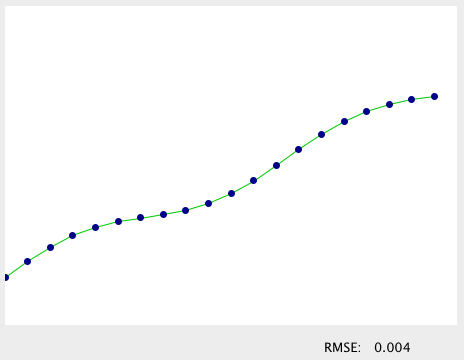
\includegraphics[width=4.5in]{figNNvalidation.png}
    \caption{Target values (blue dots) versus values predicted (green line) by a neural network with one input, one output, and five hidden units on a simple test function.}
    \label{figNNvalidation}
  \end{center}
\end{figure}

With a neural network implementation in hand, we can now turn to the CellMLNeuralNet class, which predicts cell state from a neural network.  Like CellMLDecisionTree, this class derives from CellMLSampler, providing it with a convenient numerical description of the game state via the MakeSample method.  The NextType method uses this to look up the prediction of the network, if we have one:

\begin{lstlisting}
Function NextType(extState As ExtendedState, act As Action) As CellType.Codes
  if Net is nil then
    // No memory for this location. Go with the default
    // assumption of no state change.
    return Super.NextType(extState, act)
  end if
  
  // Otherwise, use the neural net to guess the new state of this cell.
  Dim sample As NPMatrix = NPMatrix.RowMatrix( MakeSample(extState, act) )
  Dim output As NPMatrix = Net.Output(sample)
  
  // Find the output with the greatest value, and take that as our guess.
  Dim bestValue As Double = 0.0
  Dim bestCol As Integer = -1
  for col as Integer = 0 to output.Columns-1
    Dim val As Double = output.Element(0, col)
    if val > bestValue then
      bestValue = val
      bestCol = col
    end if
  next
  if bestCol < 0 then return Super.NextType(extState, act)
  return mOutColumnToType.Value(bestCol)
End Function
\end{lstlisting}

The prediction is taken as the output with the greatest value, mapped to an actual cell type via the mOutColumnToType dictionary.  That dictionary, and the network itself, are set up in the Train method, shown below.

\begin{lstlisting}
Sub Train(prevState As ExtendedState, action As Action,
          newState As ExtendedState)
  Dim prevType As CellType.Codes = prevState.state.cell( _
       mPosition.X, mPosition.Y, mPosition.Z)
  Dim newType As CellType.Codes = newState.state.cell( _
       mPosition.X, mPosition.Y, mPosition.Z)
  if newType = prevType and Net is nil then
    // Common case: the type didn't change, and we didn't expect it to,
    // because we have no changes at all stored for this cell.
    return
  end if
  
  Dim sample() As Double = MakeSample(prevState, action)
  
  // Rebuild our output matrix, assigning one column to each type we've seen.
  Dim newOutCol As Integer = mOutTypeToColumn.Lookup(newType, -1)
  if newOutCol < 0 then
    // This new type isn't one we've seen before.  We'll need to throw out
    // our old network and build a new one, with more outputs.
    Net = nil
    Dim newCol As Integer = mOutTypeToColumn.Count
    mOutTypeToColumn.Value(newType) = newCol
    mOutColumnToType.Value(newCol) = newType
  end if
  mOutTypes.Append newType
  Dim outRows As Integer = mOutTypes.Ubound + 1
  Dim outCols As Integer = mOutTypeToColumn.Count
  mOutputs = New NPMatrix(outRows, outCols)
  for row as Integer = 0 to outRows-1
    for col as Integer = 0 to outCols-1
      mOutputs.Element(row, mOutTypeToColumn.Value(mOutTypes(row))) = 1.0
    next col
  next row
  // Append the new sample to our training data
  if mInputs is nil then
    mInputs = NPMatrix.RowMatrix(sample)
  else
    mInputs.AppendRow sample
  end if
  
  // If we don't have enough inputs or outputs yet, don't attempt to 
  // train a network (it would blow up in standardization, or produce
  // pointless output).
  if mInputs.Rows < 4 or mOutputs.Columns < 2 then return
  
  if Net is nil then
    // Create a new neural network
    const numHidden = 20
    Net = New NeuralNet(sample.Ubound + 1, numHidden, mOutputs.Columns)
  end if
  
  // Train the network (a small amount, since we'll train it more
  // on each subsequent turn).
  Net.Train mInputs, mOutputs, 10
End Sub
\end{lstlisting}

The first time the default (no-change) prediction fails, we start collecting samples.  Once we have several samples, we create a new NeuralNet object with 20 hidden units, and from that point on, the network is trained for 10 iterations of the SCG algorithm per turn.

The values of 20 hidden units and 10 iterations per turn were selected by trying various values, and running the AI through Level 4, one of the more challenging levels.  The results of that experiment are given in Table~\ref{netParamsTable}.  A smaller follow-up experiment was run on Level 5, using 10 training iterations per turn, but trying 5, 10, 20, and 40 hidden units.  That produced a Level 5 score of 375, 475, 500, and 500 points respectively.  Based on these results, it was decided to use 20 hidden units and 10 iterations per turn for all subsequent work.

\begin{table}
  \begin{center}
    \begin{tabular}{|l|l|l|l|}
        \cline{2-4}
        \multicolumn{1}{c|}{} & i=10 & i=20 & i=50 \\ \hline
        h=5  & 750  & 750  & 625  \\ 
        h=10 & 750  & 750  & 600  \\ 
        h=20 & 850  & 850  & 0    \\
        \hline
    \end{tabular}
    \caption{Score of the neural net AI on level 4 for various numbers of hidden units (h) and training iterations per turn (i).}
    \label{netParamsTable}
  \end{center}
\end{table}

\section{Experimental Results}

In this section, each of the eight levels will be presented, including the logic that causes dynamic changes in the environment.  The total score for each subject will be given, and any particularly interesting behaviors will be described.

\subsection{Level 1}

\begin{figure}[ht]
\begin{minipage}[t]{0.45\linewidth}
\centering
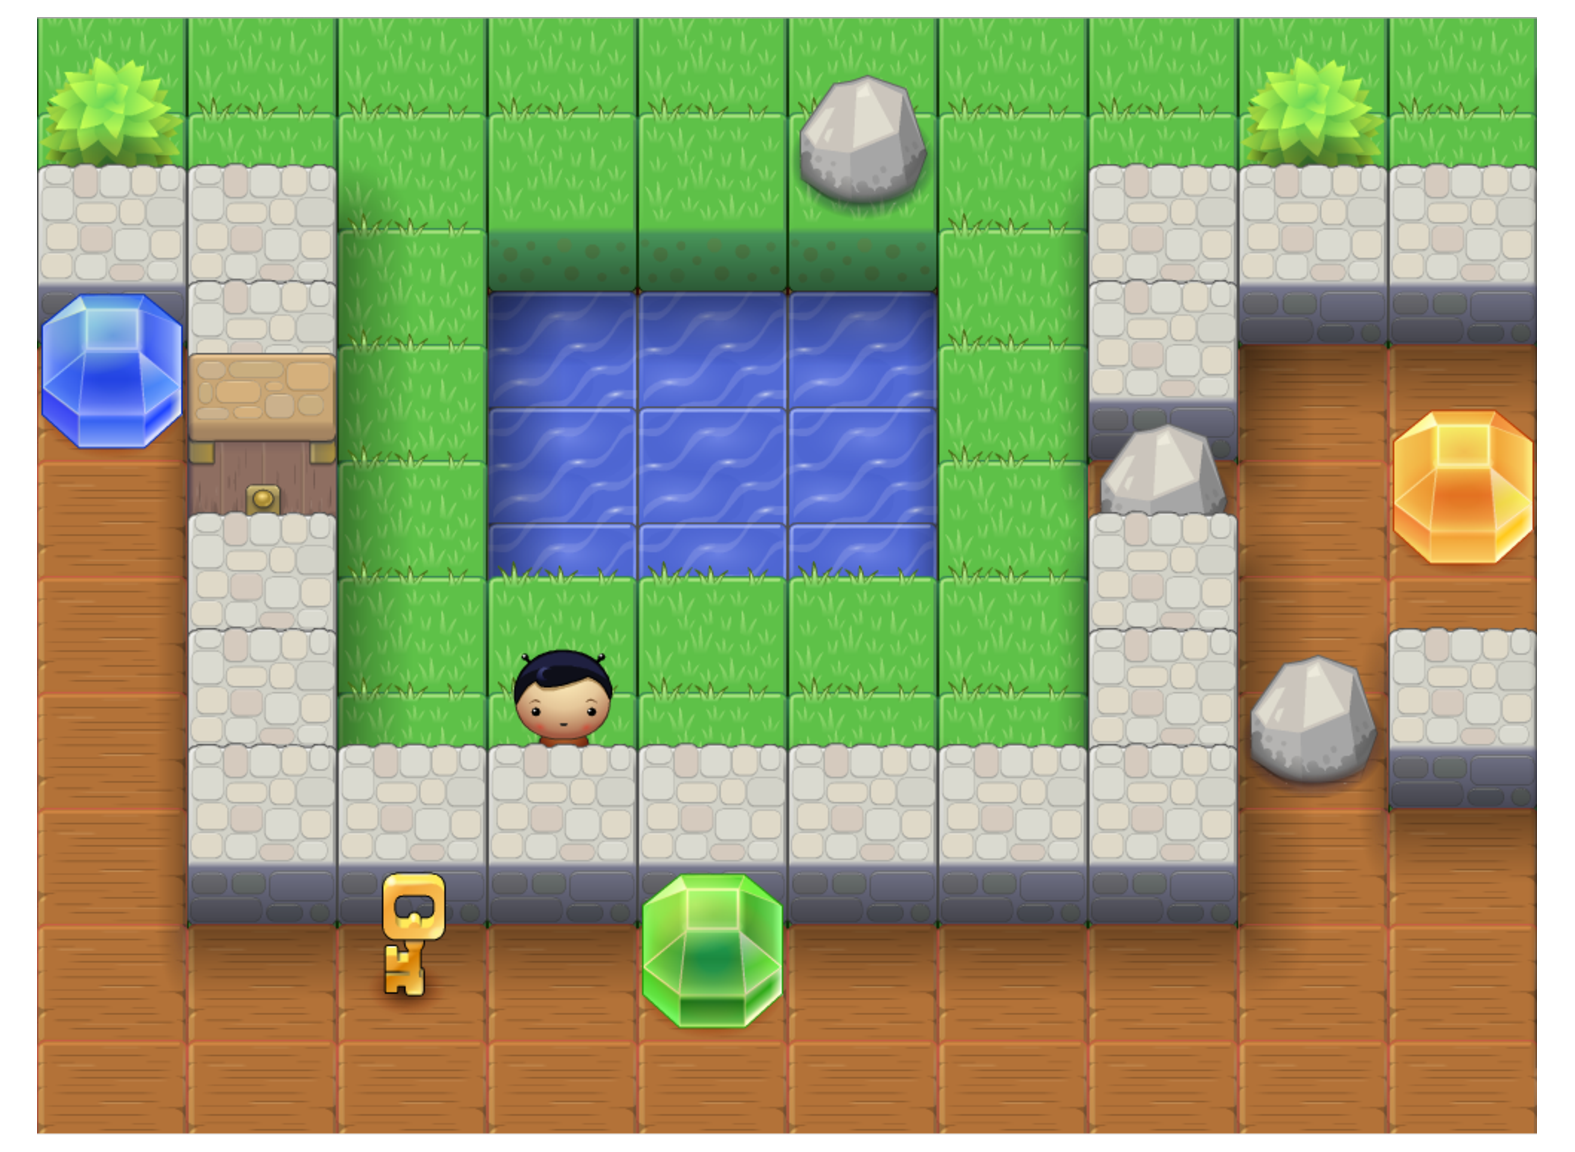
\includegraphics[width=\textwidth]{figLevel1.pdf}
\caption{Level 1. Taking any gem replaces the other two.}
\label{figLevel1}
\end{minipage}
\hspace{0.5cm}
\begin{minipage}[b]{0.45\linewidth}
\centering
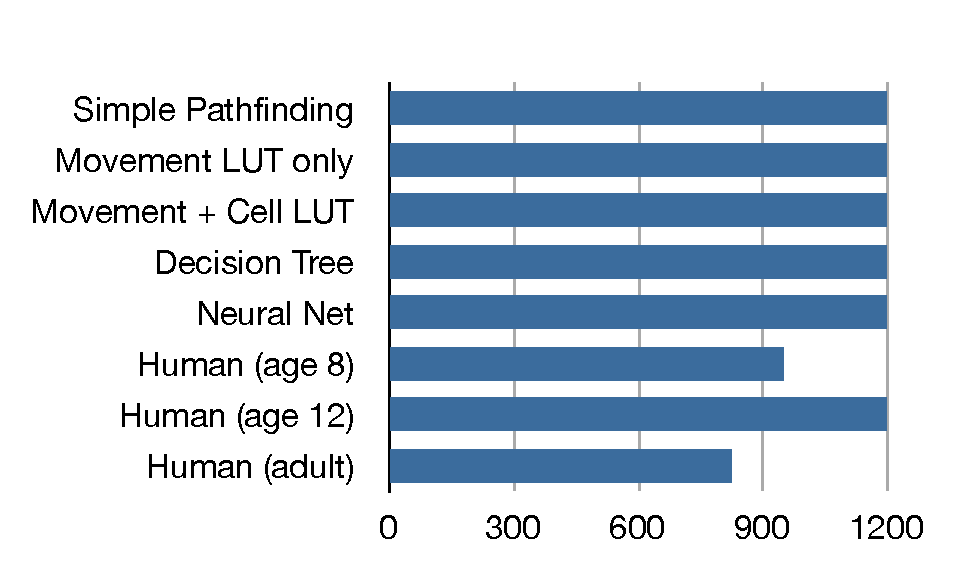
\includegraphics[width=\textwidth]{figScores1.pdf}
\caption{Subject scores on Level 1.}
\label{figScores1}
\end{minipage}
\end{figure}

The first level is shown in Figure~\ref{figLevel1}.  This first level was deliberately kept simple, with no complex level logic.  When any gem is taken, the other two gems are replaced, if they not already present; this is the only dynamic element of the level.  It does, however, present an optimization problem, as the best strategy is to ignore the key, door, and blue gem entirely, instead spending the allotted time collecting green and orange gems.  All versions of the AI went directly to this strategy, as did the 12-year-old human subject; the other two humans tried collecting the blue gem, before settling into the green-orange collection pattern.

It's worth noting that collection of the blue gem might have been a better strategy, if this had triggered some even bigger reward.  In that case, all the AIs and one of three human subjects would have missed the more profitable path.

\subsection{Level 2}

\begin{figure}[ht]
\begin{minipage}[t]{0.45\linewidth}
\centering
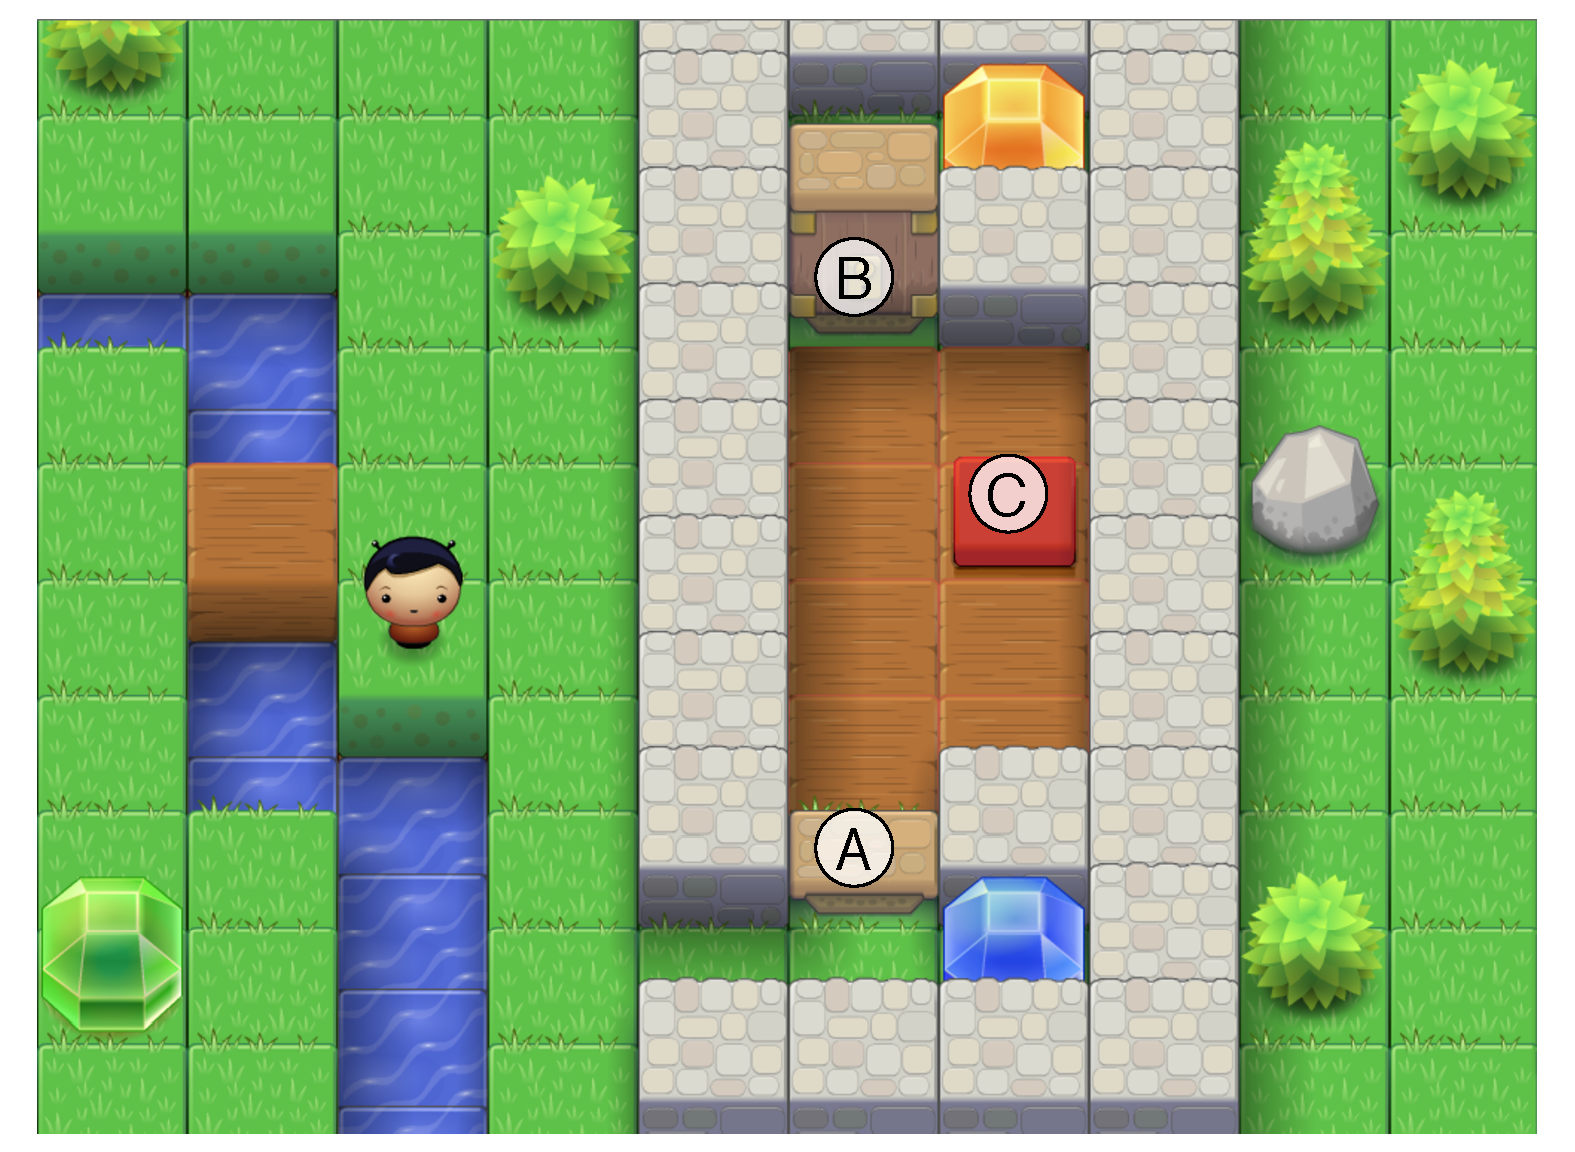
\includegraphics[width=\textwidth]{figLevel2.pdf}
\caption{Level 2.  Doors at A and B both toggle when button C is pressed; taking each gem replaces the other.}
\label{figLevel2}
\end{minipage}
\hspace{0.5cm}
\begin{minipage}[b]{0.45\linewidth}
\centering
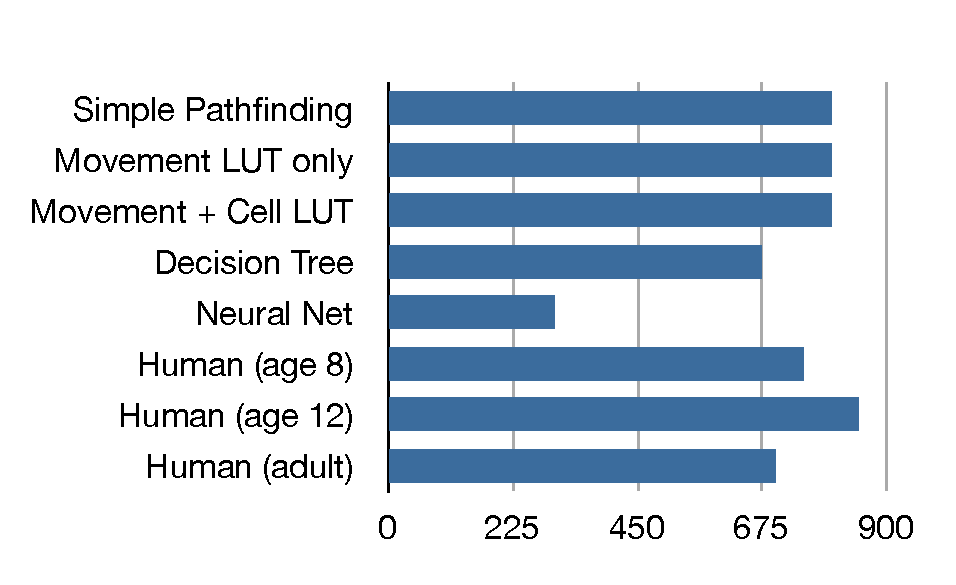
\includegraphics[width=\textwidth]{figScores2.pdf}
\caption{Subject scores on Level 2.}
\label{figScores2}
\end{minipage}
\end{figure}

The second level is shown in Figure~\ref{figLevel2}.  This level was intended to pose a challenge for straight path-finding AIs, as there is never a complete path from one gem to the other.  However, when actually tested, the non-learning AI performed near-perfectly, using the button to toggle the doors on each pass between the blue and orange gems.  This is because, once the green and blue gems had been collected, the button was the only interesting goal left, so it proceeded there.  But once the button was pressed, a path opened up to a high-value goal (orange gem).  After collecting the orange gem, the situation was similar, with the button being the only reachable goal point.

The decision tree and neural network AIs performed more poorly on this level.  Both started out behaving exactly like the non-learning AI, but once the learning algorithms kicked in, they spent a fair amount of time wandering around within the room with the button, as if experimenting to understand how it worked.  In reality, the most reasonable explanation for this behavior is that they were incorrectly predicting the state of the doors, and so believed that they had no path to the next gem, even though the door was open.  When no goals are reachable, the AI pipeline picks a move at random.  The decision tree AI went through a brief period of this confusion, and then resumed correctly navigating the level.  The neural network, on the other hand, never did manage to use the doors once it got into a confused state.

The humans all managed this level without too much trouble; the slightly lower scores of two of the human subjects represent simple missteps.  The 12-year-old subject managed to beat the AI score by ignoring the green gem and going straight for the higher-value orange gem at the start of the level, an option the AIs did not consider because there was no obvious path to it.

\subsection{Level 3}

\begin{figure}[ht]
\begin{minipage}[t]{0.45\linewidth}
\centering
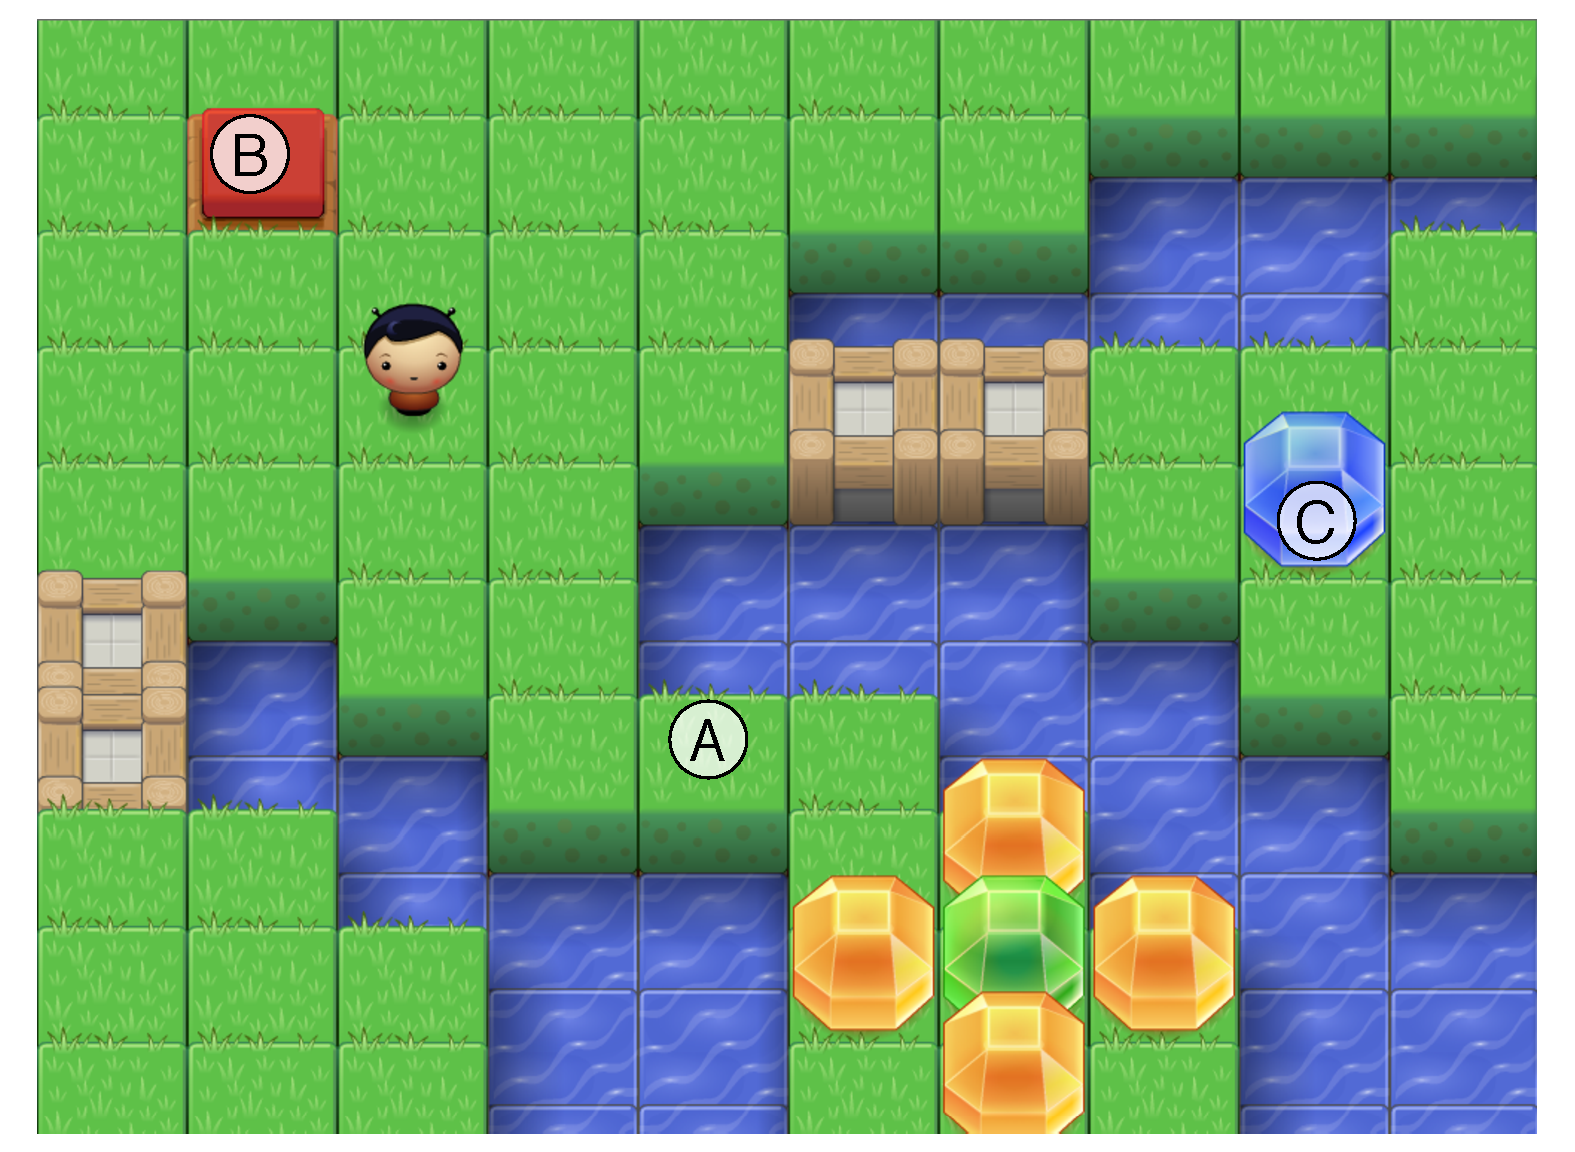
\includegraphics[width=\textwidth]{figLevel3.pdf}
\caption{Level 3.  An invisible wall at A makes it impossible to reach the green and orange gems.  Pressing button B replaces the blue gem at C.}
\label{figLevel3}
\end{minipage}
\hspace{0.5cm}
\begin{minipage}[b]{0.45\linewidth}
\centering
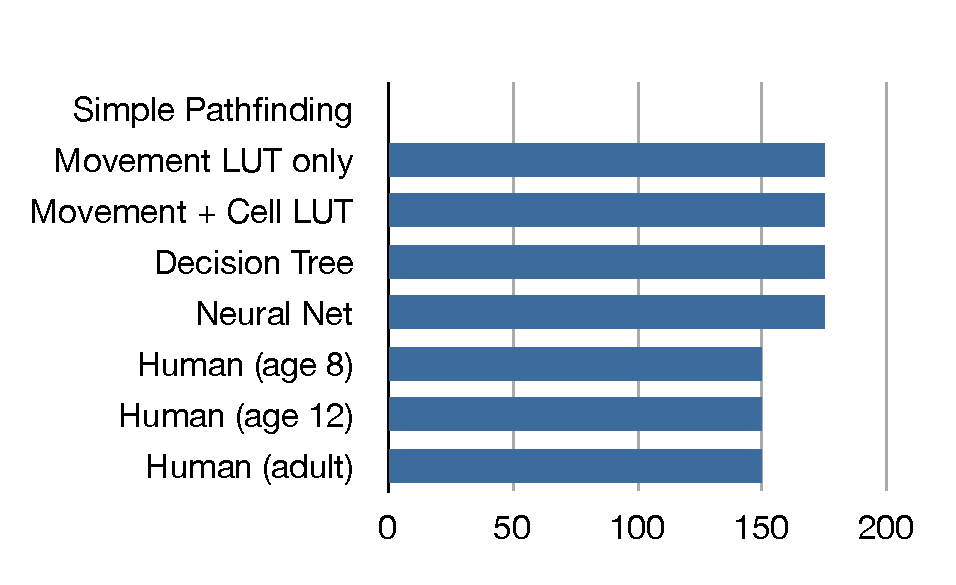
\includegraphics[width=\textwidth]{figScores3.pdf}
\caption{Subject scores on Level 3.}
\label{figScores3}
\end{minipage}
\end{figure}

The third level is shown in Figure~\ref{figLevel3}. This level contains an invisible wall, which is indistinguishable to the AI and human players from any ordinary traversable cell.  This invisible wall makes it impossible to reach a very tempting cache of high-scoring gems.  So this level amounts to a test of how quickly (if at all) each player will give up on the attractive goal when attempts to reach it fail.

As expected, the non-learning AI failed at this level completely; the agent simply tried to move into the blocked space over and over, until the time was up.  All other AIs quickly learned that that cell was impassible, and treated it as such, thanks to the MovementLUT class.  Humans took slightly longer, each trying several times, and again after pressing the button, before giving up on the high-value gems.

\subsection{Level 4}

\begin{figure}[ht]
\begin{minipage}[t]{0.45\linewidth}
\centering
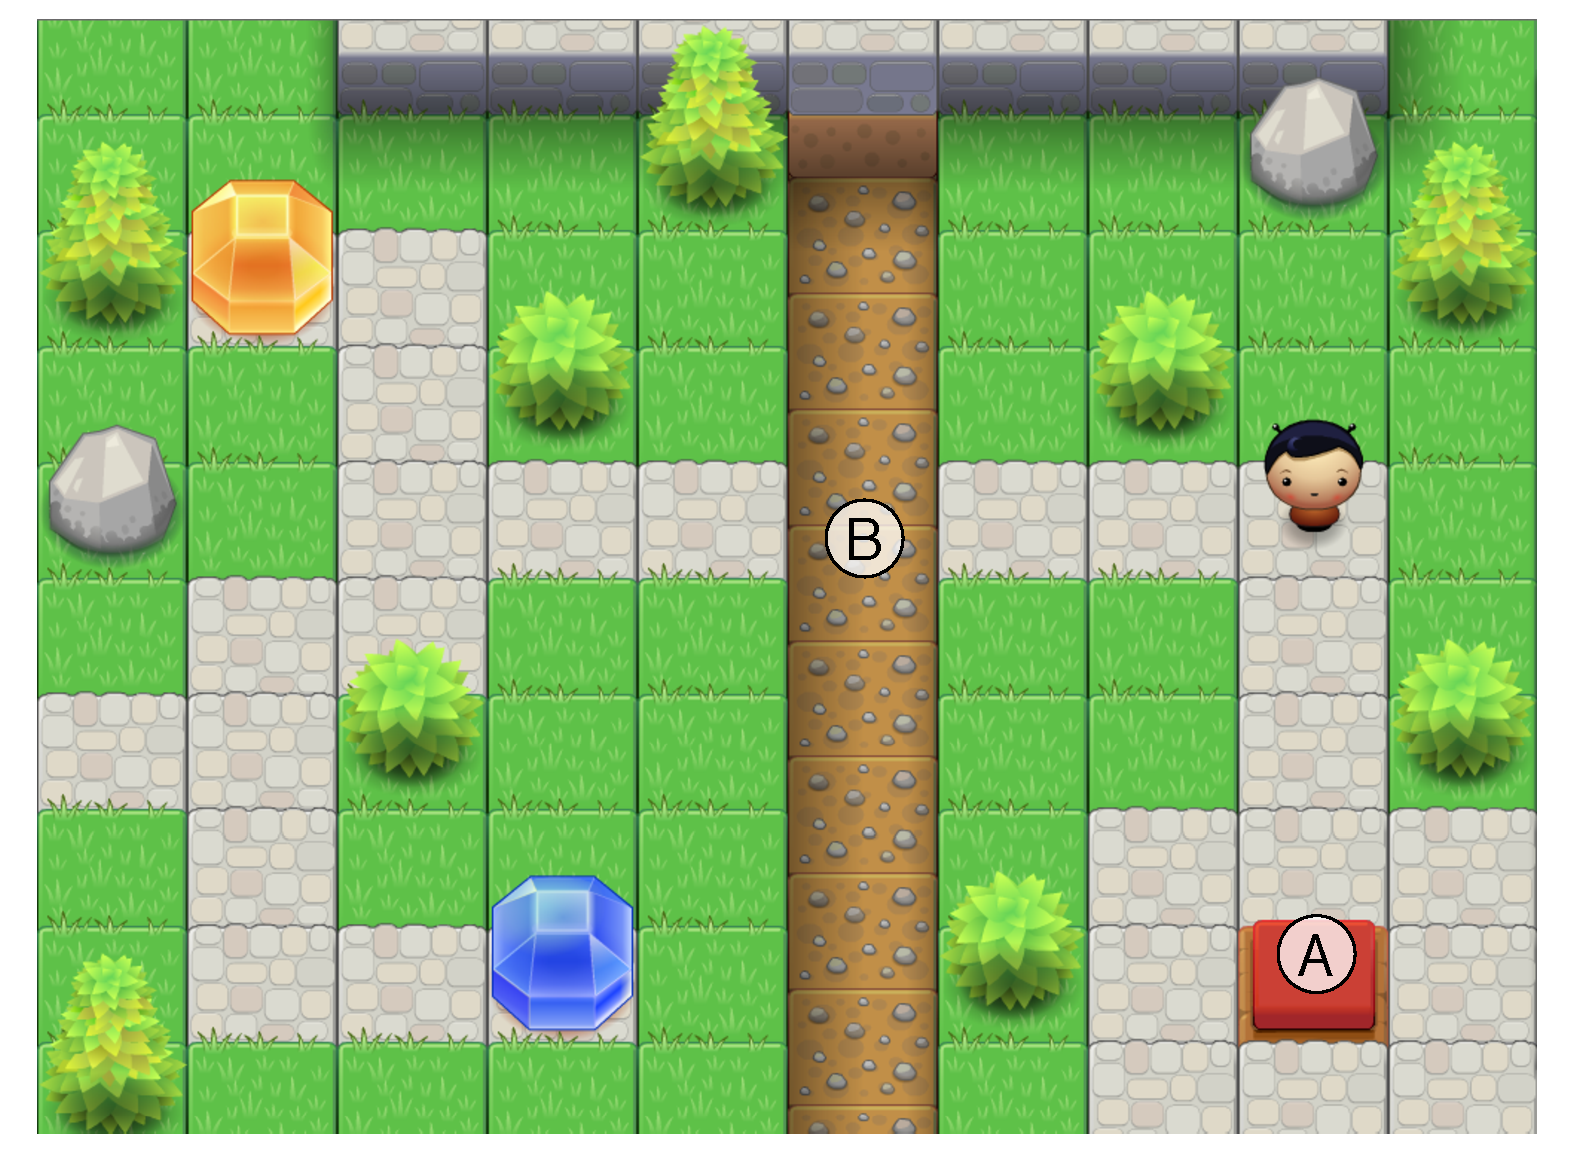
\includegraphics[width=\textwidth]{figLevel4.pdf}
\caption{Level 4. A bridge appears at point B only while button A is held down.  Taking each gem replaces the other.}
\label{figLevel4}
\end{minipage}
\hspace{0.5cm}
\begin{minipage}[b]{0.45\linewidth}
\centering
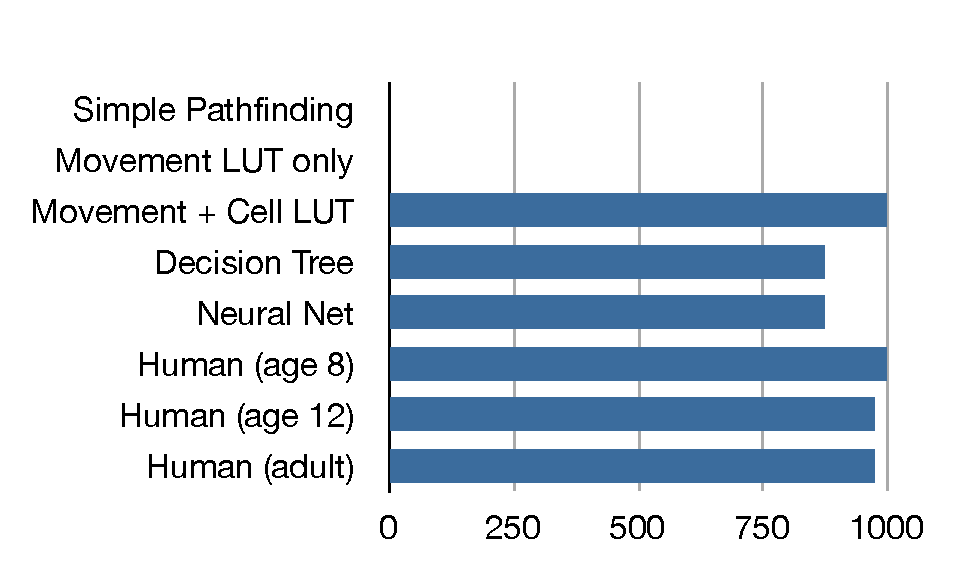
\includegraphics[width=\textwidth]{figScores4.pdf}
\caption{Subject scores on Level 4.}
\label{figScores4}
\end{minipage}
\end{figure}

Level 4 is shown in Figure~\ref{figLevel4}.  This level contains an infinite supply of gems on the left side of the board, but to get there, the player must leave a rock on the button on the right side of the board.  The score on this level essentially reflects how quickly each player managed to solve that puzzle.

The CellMLLUT AI, as well as all three humans, solved this puzzle very quickly.  The two AIs without a cell state predictor never managed to solve it at all.  Given enough time, the random action generator would probably have produced a solution for them, but this did not happen within 150 turns.

The behavior of the other two learning AIs (neural network and decision tree) was interesting.  Each of them stepped on the button, and then walked up to where the bridge had appeared, even though it was no longer there.  They then went back to the button, and stepped on and off of it in various directions, as if the direction in which you step off might make all the difference.  Only after trying all those combinations did they try dropping the rock, at which point the problem was solved, and they started collecting gems.

\subsection{Level 5}

\begin{figure}[ht]
\begin{minipage}[t]{0.45\linewidth}
\centering
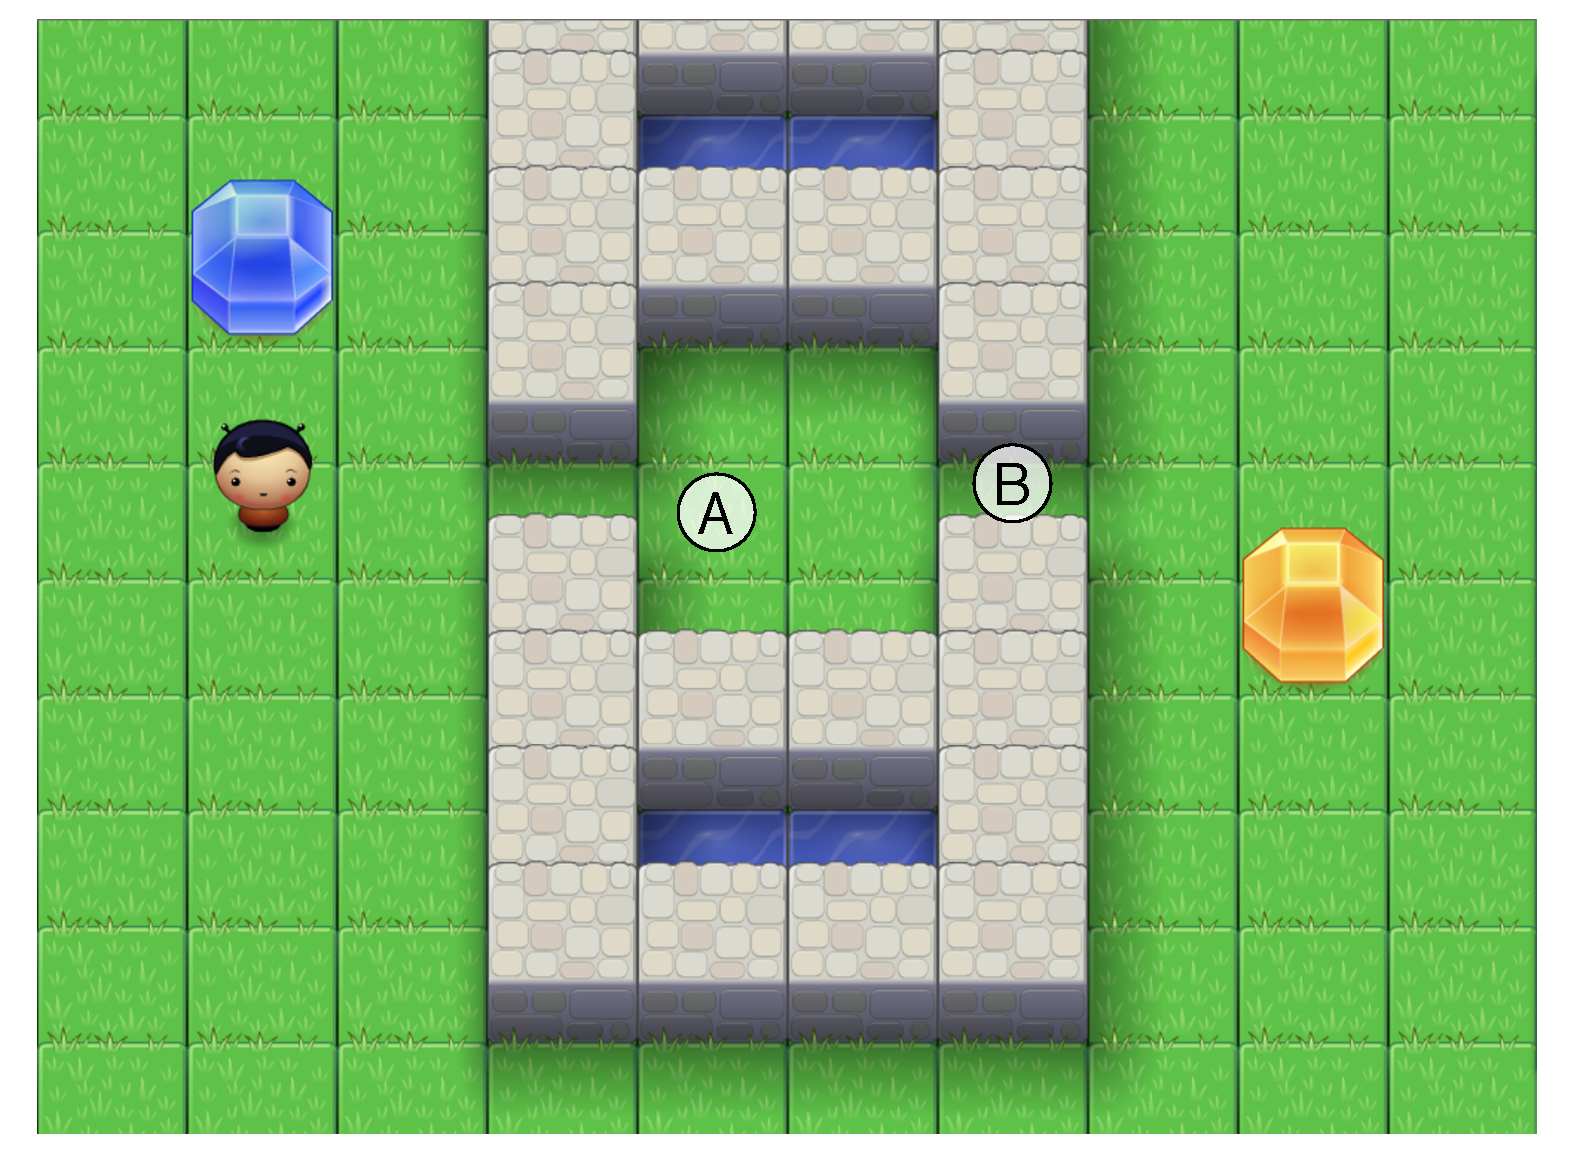
\includegraphics[width=\textwidth]{figLevel5.pdf}
\caption{Level 5.  A wall appears at point B only when the Euclidian distance from the player to point A is less than 2.  Taking each gem replaces the other.}
\label{figLevel5}
\end{minipage}
\hspace{0.5cm}
\begin{minipage}[b]{0.45\linewidth}
\centering
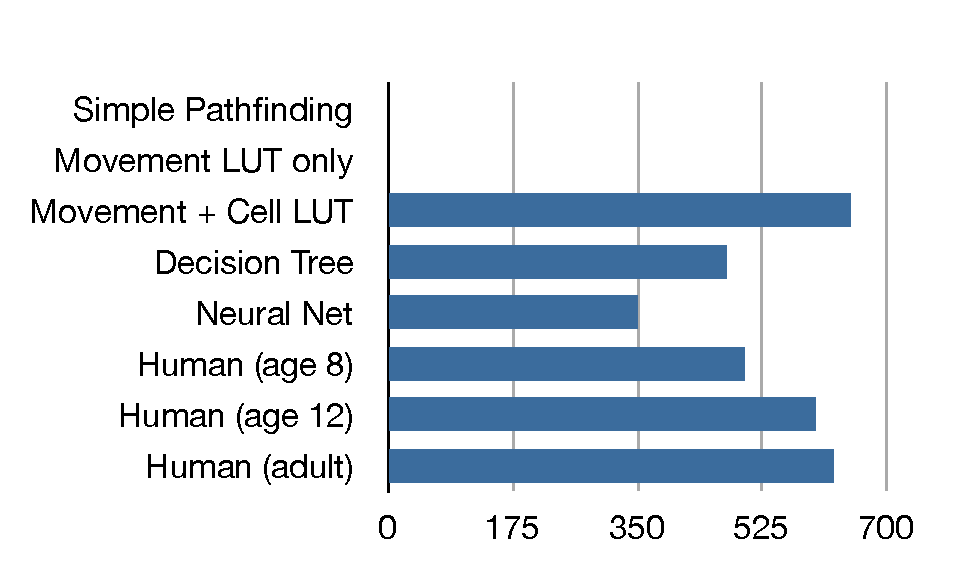
\includegraphics[width=\textwidth]{figScores5.pdf}
\caption{Subject scores on Level 5.}
\label{figScores5}
\end{minipage}
\end{figure}

The fifth level is shown in Figure~\ref{figLevel5}.  This level was described by the youngest human subject as ``mean'' because every time the player tries to take the short path through the center towards the orange gem, a wall appears, blocking his progress.  When the player moves back out of the center passage, this wall disappears.

As expected, the two simpler AIs utterly failed to solve this task.  Each would step into the center passage, find it blocked, step out, find it unblocked, and step in again, in a repeating pattern without end.  This is exactly the sort of failure that exasperates gamers when seen in NPCs.

The three more advanced AIs learned that they couldn't get through this way, and went around the long way.  The CellMLLUT (lookup table) AI learned this most quickly, and also found that the shortcut was passable in the other direction, obtaining an optimal score.  The neural network took the longest to learn, and as a result spent a fair amount of time in fruitless exploration of the central chamber.

The score of the decision tree AI was in between, because it quickly learned that it couldn't take the shortcut from left to right, but then overgeneralized, and also went the long way from right to left.  It clearly believed that if it tried to take the shortcut in the other direction, it would be blocked, so it never bothered to try.  The 8-year-old human subject did exactly the same thing.

\subsection{Level 6}

\begin{figure}[ht]
\begin{minipage}[t]{0.45\linewidth}
\centering
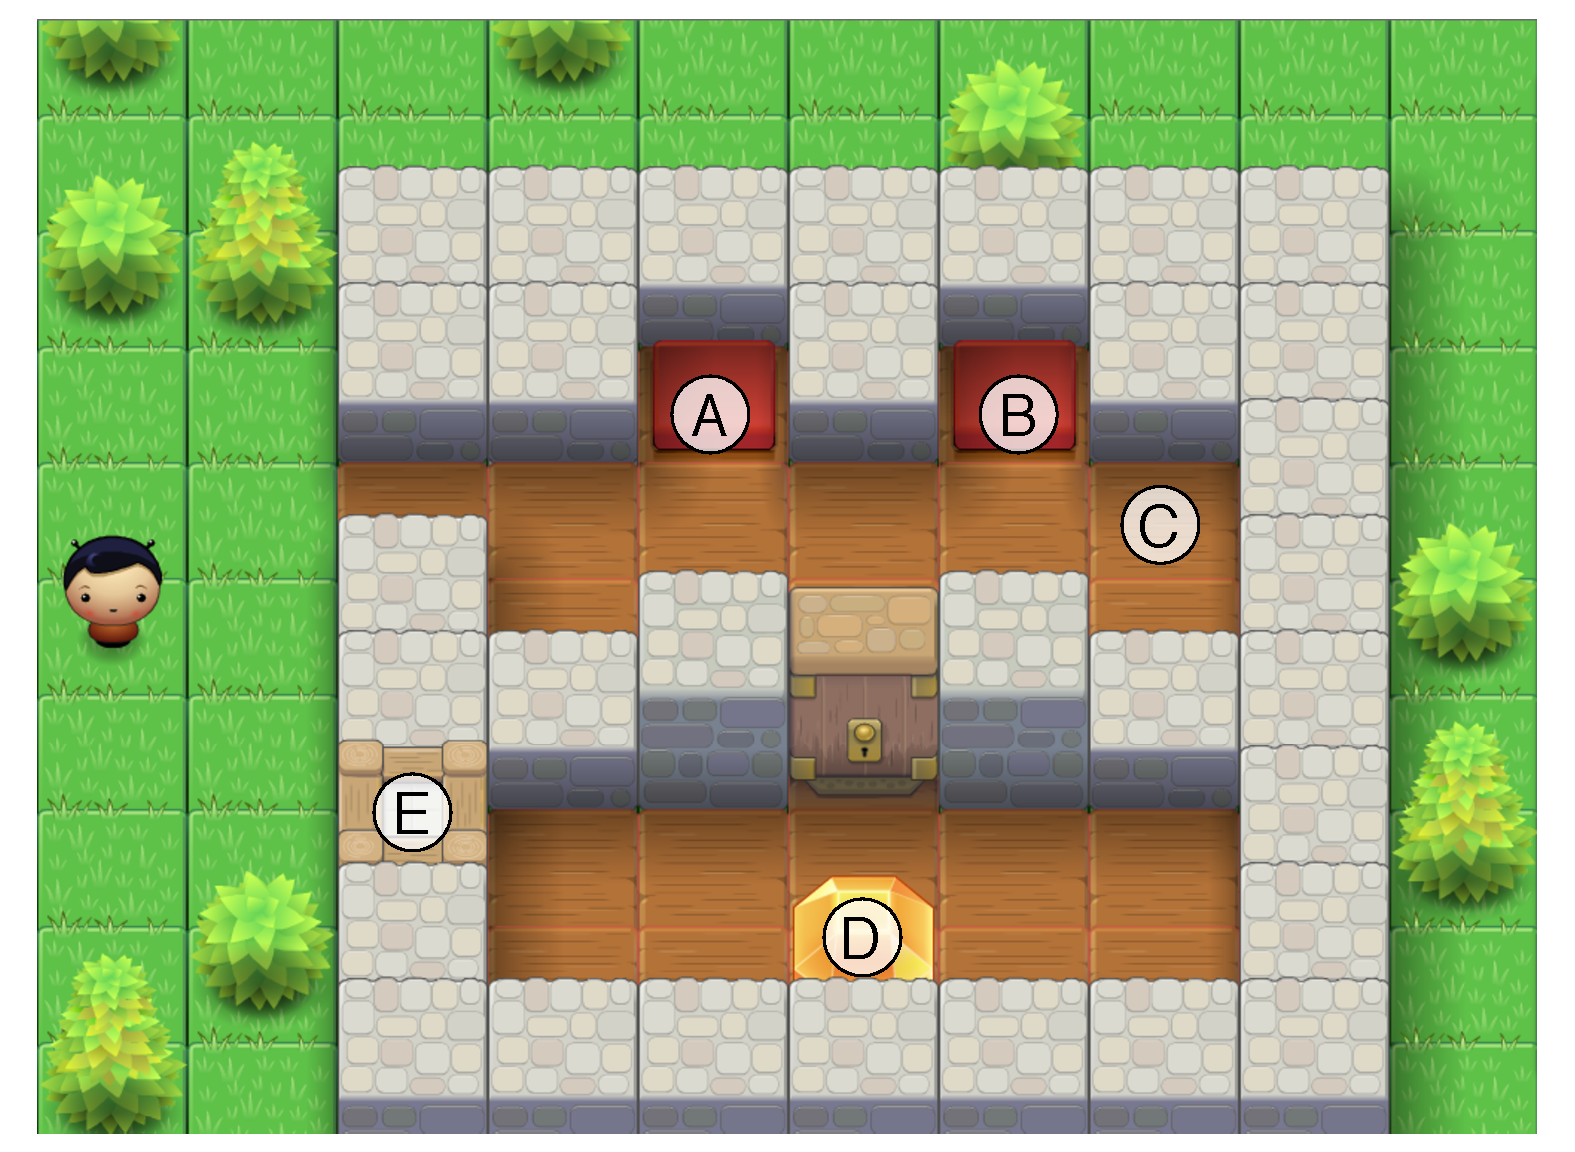
\includegraphics[width=\textwidth]{figLevel6.pdf}
\caption{Level 6. Pressing button A causes gem D to appear, and any key at C to disappear; pressing button B does the inverse.  When gem D is taken, the door is closed and wall E disappears, which then reappears as soon as the player steps through.}
\label{figLevel6}
\end{minipage}
\hspace{0.5cm}
\begin{minipage}[b]{0.45\linewidth}
\centering
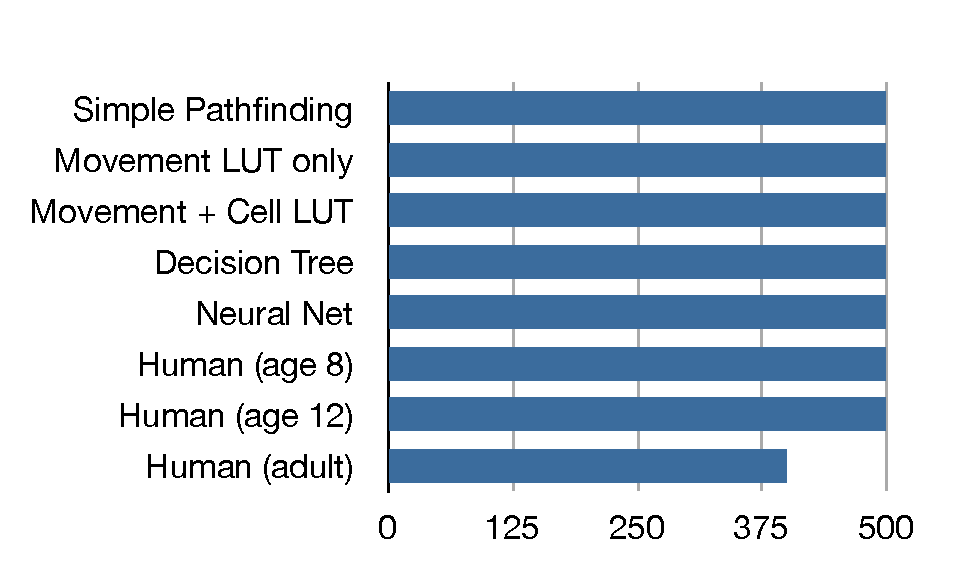
\includegraphics[width=\textwidth]{figScores6.pdf}
\caption{Subject scores on Level 6.}
\label{figScores6}
\end{minipage}
\end{figure}

The sixth level is shown in Figure~\ref{figLevel6}.  This level was intended to be difficult: to successfully collect a gem requires pressing the second (rightmost) button first, collecting the key, and only then pressing the first button to make the gem appear.

As it turned out, all AIs solved this problem immediately.  Though they did press the left button first on the first run through, when nothing happened, they proceeded to the next button.  This caused a key to appear, which is a higher-valued goal than button pressing, so it was collected.  Then, with no other reachable goals, the selection heuristics specify pressing the least recently used button, which was always the right thing to do for the rest of the level.  In short, the goal rankings, selection heuristics, and path finder combined to produce productive behavior in this case, even without machine learning.

The humans demonstrated essentially the same behavior, although the adult subject did make one round through the lower room when there was no gem to collect, perhaps just to see what would happen.

\subsection{Level 7}

\begin{figure}[ht]
\begin{minipage}[t]{0.45\linewidth}
\centering
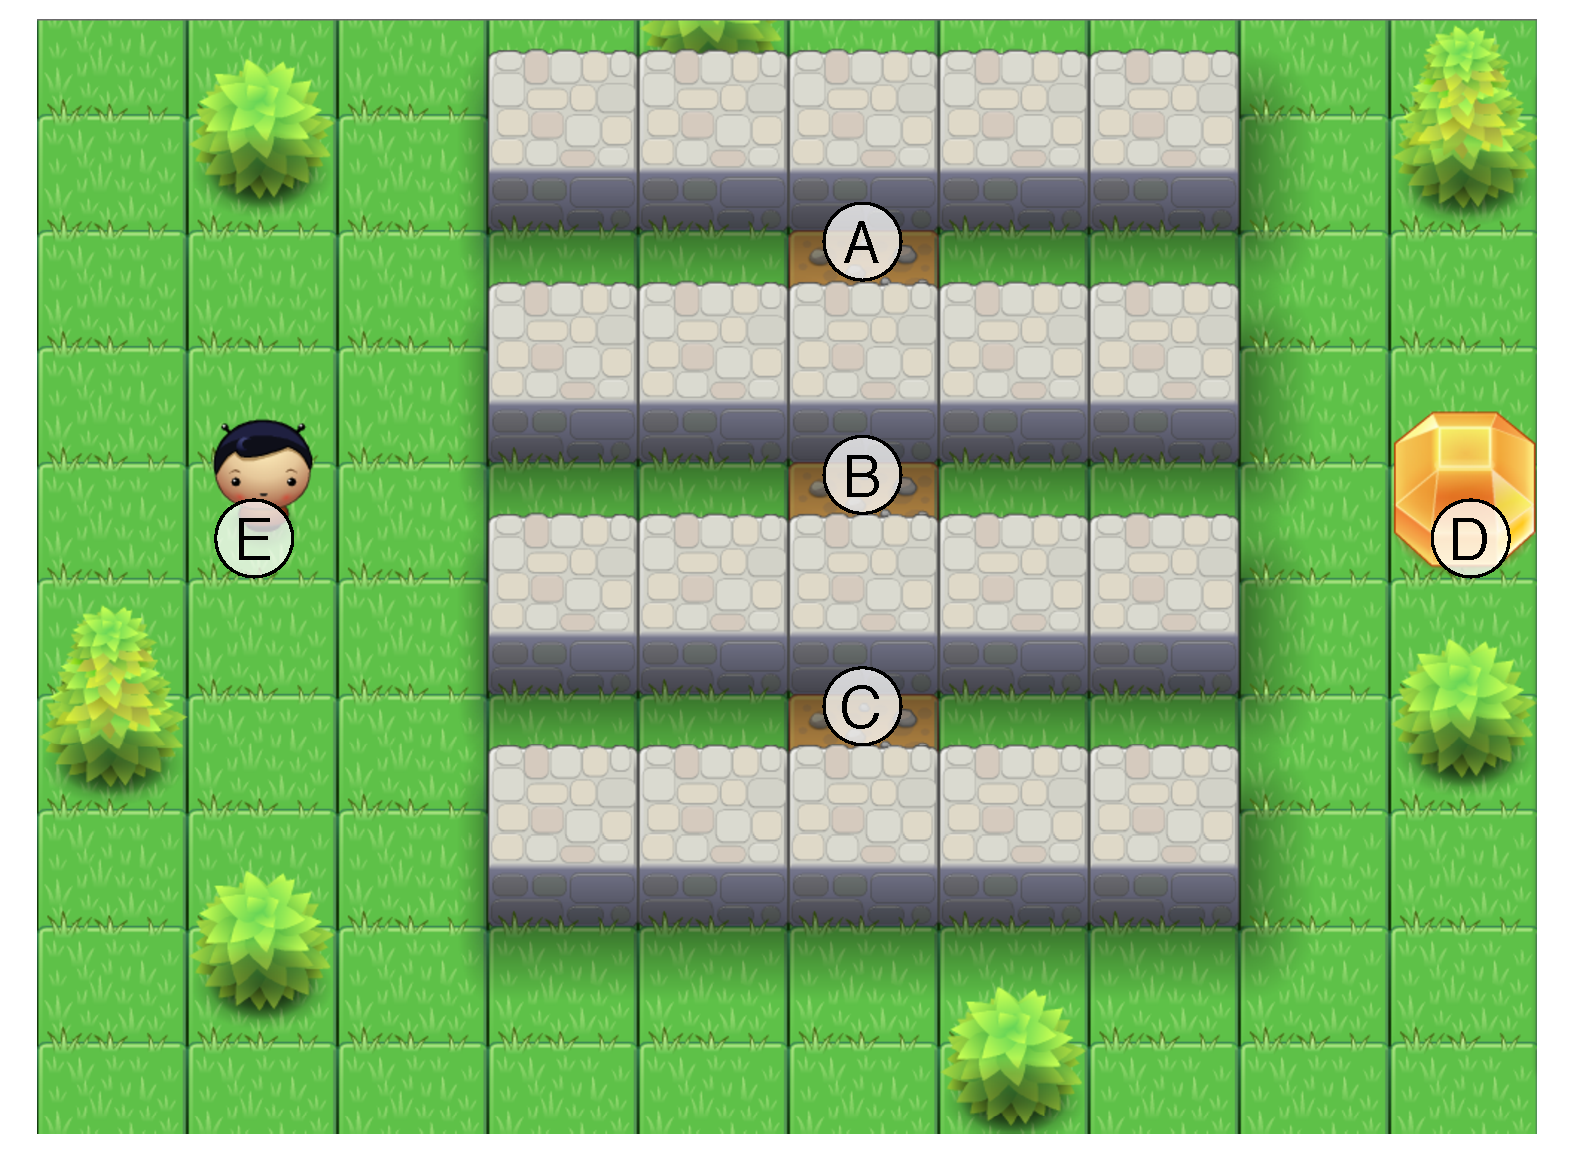
\includegraphics[width=\textwidth]{figLevel7.pdf}
\caption{Level 7. Walls at A, B, and C appear and disappear with different periods.  Taking the gem at D replaces one at E, and vice versa.}
\label{figLevel7}
\end{minipage}
\hspace{0.5cm}
\begin{minipage}[b]{0.45\linewidth}
\centering
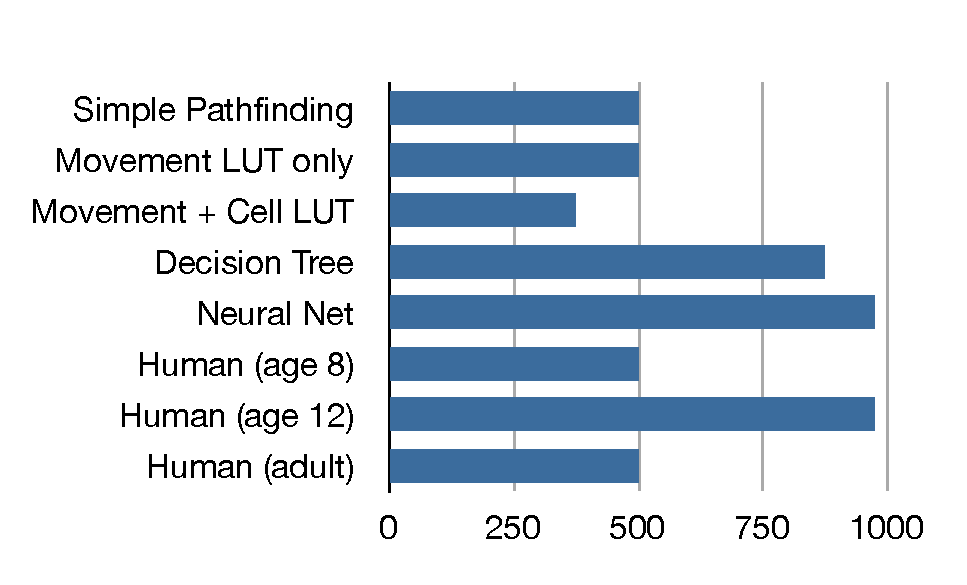
\includegraphics[width=\textwidth]{figScores7.pdf}
\caption{Subject scores on Level 7.}
\label{figScores7}
\end{minipage}
\end{figure}

The seventh level is shown in Figure~\ref{figLevel7}.  In this level, three useful passages are periodically blocked, by walls that appear and disappear strictly by the turn counter.  As a result, passage A in the figure is passable for 2 turns, and blocked for 2 turns; B is passable for 3 turns, and blocked for 4 turns; and C is passable for 4 turns, and blocked for 6 turns.

This level produced a wide range of scores in both AIs and human subjects.  This was the only level in which the CellMLLUT (lookup table) AI got the worst score.  At the risk of anthropomorphizing, its behavior might be described as ``flustered,'' making multiple attempts on each trip to get through the passages, and then giving up, in some cases even when the path was actually clear.

The non-learning AIs did slightly better; they simply turned around every time the chosen passage was blocked, but this led them to a working passage often enough to get a somewhat higher score.

The decision tree AI performed substantially better; it seemed to correctly predict the obstacles, and sometimes took the upper passage, or made a few extra moves in order to reach the barriers just as they disappeared.  The best performance, however, was from the neural network AI.  It simply went back and forth through the middle passage, waiting (by running into the wall) a turn or two as needed.  This was the only level in which the neural network outperformed the decision tree AI.

Behavior of the human subjects was very interesting.  The youngest never even attempted the central passages, but instead went the long way around every time.  The adult subject tried the central passages several times, ran into a wall, and then gave up and went the long way for the rest of the level.  One might speculate that these subjects never realized the periodic nature of the obstacles, instead forming a mental model similar to Level 5, where the level logic was purposely thwarting them.  The 12-year-old human subject, however, quickly realized the nature of the walls, and selected the same solution as the neural network.

\subsection{Level 8}

\begin{figure}[ht]
\begin{minipage}[t]{0.45\linewidth}
\centering
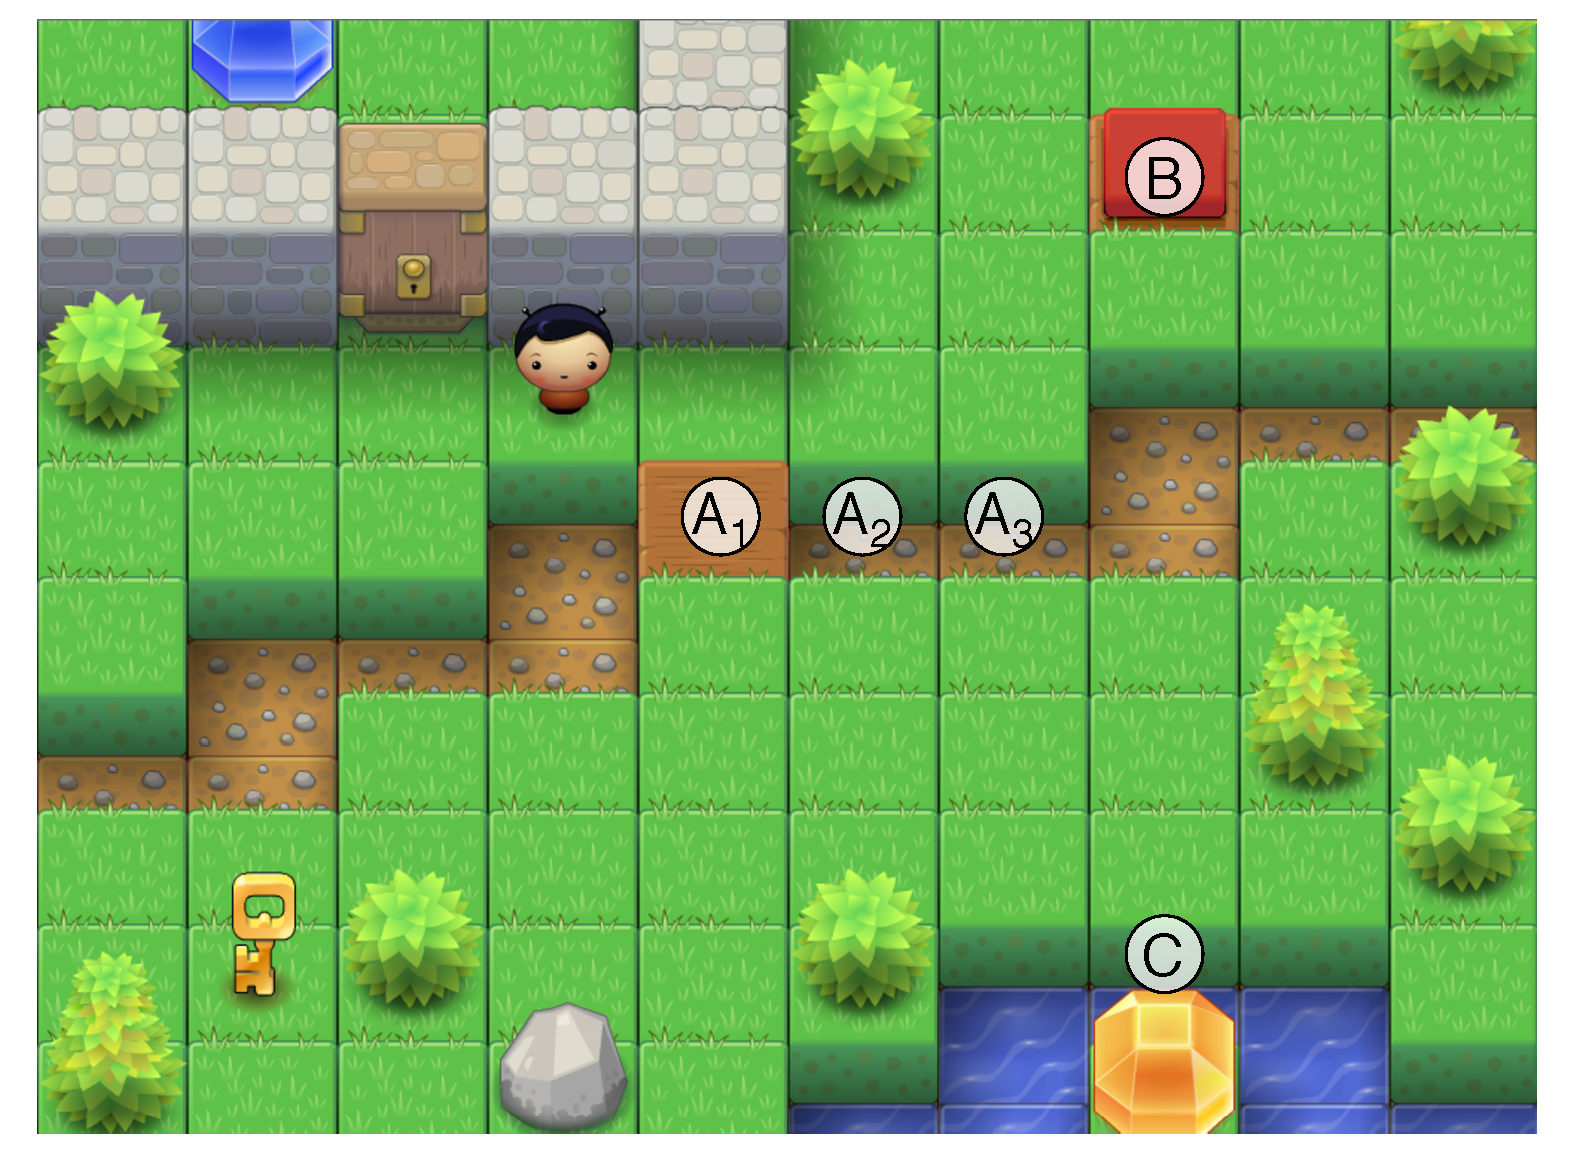
\includegraphics[width=\textwidth]{figLevel8.pdf}
\caption{Level 8. The wooden bridge moves every two turns in the pattern A1, A2, A3, A2.  Another bridge appears at point C only when button B is held down.  Taking each gem replaces the other.}
\label{figLevel8}
\end{minipage}
\hspace{0.5cm}
\begin{minipage}[b]{0.45\linewidth}
\centering
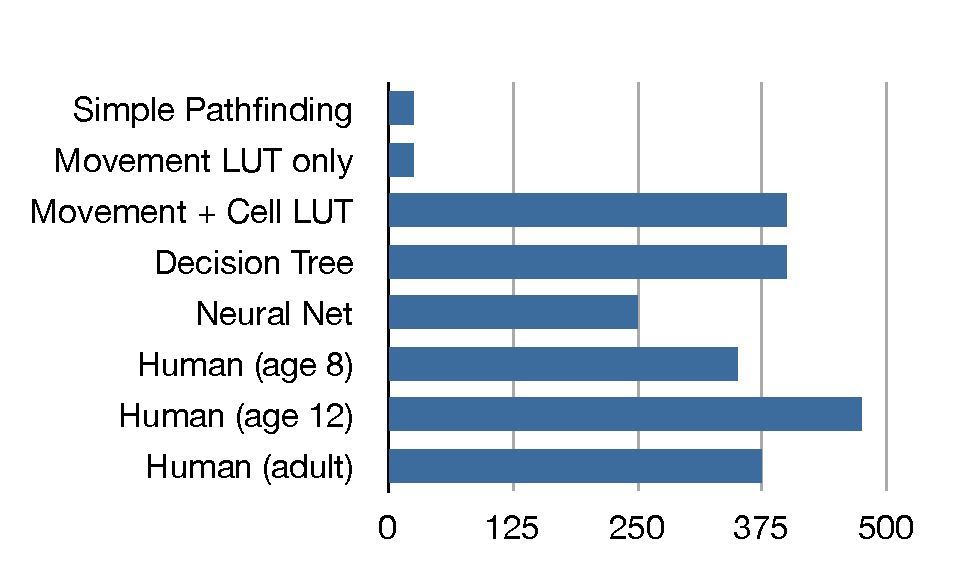
\includegraphics[width=\textwidth]{figScores8.pdf}
\caption{Subject scores on Level 8.}
\label{figScores8}
\end{minipage}
\end{figure}

The final level is shown in Figure~\ref{figLevel8}.  This level was intended to recap many of the challenges of previous levels, providing an overall gauge of performance in one level.  Full success requires using a key to open a door, using a rock to hold down a button, and navigating a moving bridge.

The two AIs without a cell state predictor managed to navigate the bridge and collect the blue gem, but as in Level 4, could not solve the rock-on-button puzzle to score any further points.  The other AIs performed well; the decision tree and lookup table versions surpassed two out of three human subjects.  The neural network struggled with the button puzzle, spending a lot of time stepping on and off the button before finally placing down a rock.


\subsection{Total Scores}

\begin{figure}
  \begin{center}
    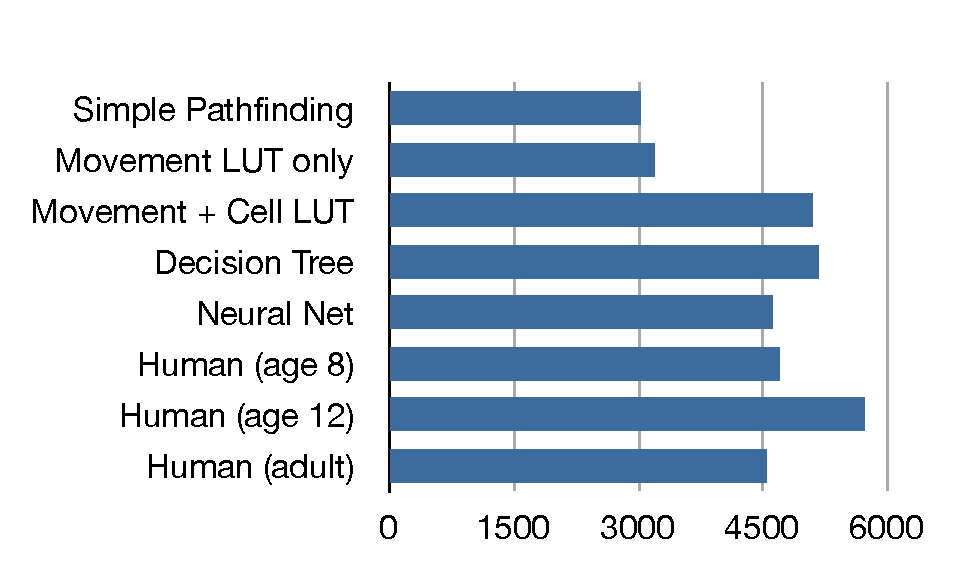
\includegraphics[width=4.5in]{figTotalScores.pdf}
    \caption{Total scores over all eight levels.}
    \label{figTotalScores}
  \end{center}
\end{figure}

Final scores for all eight subjects are shown in Figure~\ref{figTotalScores}.  The shortcomings of the simple pathfinding AI, compared to human subjects or more advanced AIs, can clearly be seen.  Adding the movement predictor helps avoid getting stuck on unexpected obstacles, such as invisible walls, but does not provide any benefit to dealing with dynamic changes in the environment.

The three versions of the AI with a cell state predictor all performed within the range of human performance.  The lookup table and decision tree AIs scored higher than two of the three human subjects.

\section{Discussion}

This project explored the use of machine learning to enable non-player characters to cope with a dynamic environment.  Full AIs based on lookup tables, decision trees, or neural networks were compared with two more limited AIs, and three human subjects.

The neural network and decision tree both act on the same feature vectors, making their results directly comparable.  The cell state predictor based on lookup tables (CellMLLut) is slightly different.  Because the dictionary used for the lookup table is based on string keys, it uses a compressed representation of the full map state, without clock features; whereas the decision tree and neural network saw only selected points in the map, but had access to the clock.  This difference could account for the lookup table's poor performance in Level 7.  On the other hand, the clock features could be confounding factors that make learning more challenging for a lookup table in other cases.  Future work should remove this variable by making a lookup table predictor that uses the same features as the other AIs.

Neural networks are well suited to dealing with continuous and potentially noisy signals.  In a clean environment like this, described by integer positions and states, it's not clear that neural networks have a distinct advantage over decision trees.  An advantage might be found in cases where a nonlinear combination of attributes is needed to predict an output; in such cases, a decision tree would need many examples and a complex tree to approximate the function.  However, in this project at least, such situations appear to be rare; the decision tree's performance was substantially better than the neural network.

The high performance of the AI based solely on lookup tables was surprising.  It equalled or outperformed the decision tree on every level except Level 7.  The lookup table approach was included essentially as another control; I expected it to be inflexible and inadequate for the complex environment in this project.  But as Ross Beveridge observed, ``Memorizing the answers is a pretty good way of knowing the answers''~\cite{ROSSCHAT}.  Though care must be taken to define a useful feature vector, lookup tables can be a powerful, efficient approach to learning that deserves more consideration in future projects.

One important difference between human subjects and the AIs in this study is that the latter retained no memory between levels.  The geometry of each level is completely different, but humans are likely to retain general principles such as ``an obvious shortcut is probably not going to work'' or ``placing a rock on a button may be useful.''  AIs that could learn such general principles, and apply them in new contexts, would appear even more humanlike, and might have a noticeable advantage over AIs without such memory.  This remains an exciting area for future research.


\bibliography{cs545final}
\bibliographystyle{plain}

\end{document}

